\documentclass{article} %llncs
\usepackage[T1]{fontenc}
\usepackage[utf8]{inputenc}

%% \usepackage{fontspec}
%% \newfontfamily{\tam}[Script=Tamil]{Lohit Tamil}
%% \defaultfontfeatures{Scale=MatchLowercase}

\usepackage{eurosym}
\usepackage{hyperref}		% clickable references
\usepackage{url}
\usepackage{apacite}            % APA style citations

\usepackage{amsmath,amssymb}	% math structures and symbols
\usepackage{graphicx}		% including of graphics files in various formats
\usepackage{amsfonts}
\usepackage{dialogue}
\usepackage{placeins}
\usepackage{tikz}
\usetikzlibrary{positioning,backgrounds,fit,arrows,shapes,shadows}
\usetikzlibrary{shapes.multipart}
\usepackage{wrapfig}
\usepackage{enumitem}
\usepackage{framed}

% \hypersetup{hidelinks}

\usepackage[xspace,mla]{ellipsis}

\definecolor{myyellow}{RGB}{242,226,149}
\definecolor{mygreen}{RGB}{144,238,144}
\definecolor{mypink}{RGB}{255,182,193}
\definecolor{myorange}{RGB}{255,165,0}
\definecolor{myblue}{RGB}{0,204,204}

\usepackage{xparse}
\NewDocumentCommand\StickyNote{O{4cm}mmO{4cm}}{%
\begin{tikzpicture}
\node[
drop shadow={
  shadow xshift=2pt,
  shadow yshift=-4pt
},
inner xsep=7pt,
fill=#2,
xslant=-0.05,
yslant=0.05,
inner ysep=10pt
] {\parbox[t][#1][c]{#4}{#3}};
\end{tikzpicture}%
}

%\urldef{\mailsa}\path|{j.corneli,s.colton}@gold.ac.uk|
%\urldef{\mailsb}\path|a.pease@dundee.co.uk|

\newcommand{\keywords}[1]{\par\addvspace\baselineskip
\noindent\keywordname\enspace\ignorespaces#1}

\begin{document}

% TITLE INFORMATION
%% \title{Modelling serendipity in a computational context}
%% \author{Joseph Corneli\inst{1}, Alison Pease\inst{2}, Simon Colton\inst{1},\\ Anna Jordanous\inst{3}, Christian Guckelsberger\inst{1}}
%% \date{\today}
%% \institute{Department of Computing, Goldsmiths College, University of London\\
%% %% \mailsa\\
%% %% \mailsb\\
%% % \url{http://ccg.doc.gold.ac.uk/}
%% \and
%% School of Computing, University of Dundee
%% \and
%% School of Computing, University of Kent}

%% \maketitle

\begin{abstract}
Most prior work that deals with serendipity in a computing context focuses on computational ``discovery''; we argue that serendipity also includes an important ``invention'' aspect.
Building on a survey that describes serendipitous discovery and invention in science and technology, we advance a definition of serendipity and an accompanying model that can be used evaluate the potential for serendipity in computational systems.  The model adapts existing recommendations for evaluating computational creativity.
It is applied in three case studies that evaluate the serendipity of existing and hypothetical systems in the context of
evolutionary computing, recommender systems, and automated programming.
From this analysis, we extract recommendations for practitioners working with computational serendipity, and outline future directions for research.  We argue there is much to be gained by creating systems with the potential for serendipity, and that serendipity is particularly critical for autonomous systems.
\\[.3cm]

\keywords{serendipity, evaluation, computational creativity, autonomous systems}
\end{abstract}


\tableofcontents

\section{Introduction}

Materials, like gold, and processes, like metalurgy, have no value
without a context of application: decoration, trade, circuitry, and so
on.  In practice, we are likely to attribute \emph{value} to materials that
are useful, and \emph{creativity} to a person who puts materials to use in a
novel way.
%
Many instances of \emph{serendipity} centre on reevaluation.  For
example, a non-sticky ``superglue'' that no one was quite sure how to
use turned out to be just the right ingredient for 3M's
Post-it\texttrademark\ notes.
%
Serendipity is related, firstly, to deviations from familiar patterns,
and secondly, to new insight.
%
When we consider the practical uses for weak glue, the possibility
that a life-saving antibiotic might be found growing on contaminated
petri dishes, and or the idea that cockle-burs could be anything but
annoying, we encounter radical changes in the evaluation of what's
interesting.  In the \emph{d\'enouement}, what was initially
unexpected is found to be both explicable and useful.

Van Andel \citeyear{van1994anatomy} -- echoing Poincar\'e's
\citeyear{poincare1910creation} (negative) reflections on the potential
for a purely computational approach to mathematics -- claimed that:
\begin{quote}
``\emph{Like all intuitive operating, pure serendipity is not amenable
    to generation by a computer.  The very moment I can plan or
    programme `serendipity' it cannot be called serendipity
    anymore}.'' \cite{van1994anatomy}
\end{quote}
We believe that serendipity is not so mystical as such statements
might imply, and in Sections \ref{sec:patterns-of-serendipity} and
\ref{sec:computational-serendipity} we will show how it is possible to
reinterpret van Andel's ``patterns of serendipity'' in computational
settings.  

The real problem with computers is not that they only do what they're
told, but that the act of programming forces us to confront the
emergence of the new \cite{mead1932philosophy}.
%
Minsky \citeyear{minsky1967programming} suggests that in practice,
programmers write programs ``for the individuals of little societies''
precisely because we cannot envision in advance all of the details of
program interactions.
%
Indeterminacy forms an important part of any proposal for
``intelligent machines'', after Turing:
\begin{quote}
``\emph{They will make mistakes at times, and at times they may make
    new and very interesting statements, and on the whole the output
    of them will be worth attention to the same sort of extent as the
    output of a human mind}.''  \cite{turing-intelligent}
\end{quote}

Serendipity has played a role in the large-scale history of the
computing field \cite{de2013turing} and in artistic applications of
computer technology \cite{reichardt1969cybernetic}.  We aim to clarify
the role it has to play in the future development of computational
creativity.

Whereas van Andel speaks of ``patterns of serendipity'' in a
relatively informal way, this paper will rely on the somewhat more
formal theory of \emph{design patterns} \cite{alexander1999origins},
to which it makes several additions and alterations.  This theory is
by no means limited to computing, and indeed, has its origins in
architecture and urban planning.  Our approach to ``designing for
serendipity'' \cite{andre2009discovery} centres on the use of design
patterns to capture the dynamic aspects of serendipitous situations.

The typical use of design patterns, since they were introduced by
Christopher Alexander
\cite{alexander1979timeless,alexander1977pattern}, is to prescribe as
well as to describe.  Design patterns provide models \emph{for} as
well as models \emph{of} \cite<cf.>[p. 93]{geertz1973interpretation}.
Thus, when Alexander describes the pattern \emph{A place to wait}, he
is telling readers that it is a good idea to consider building such
places when designing living spaces.  In connection with our
understanding of serendipity as closely associated with deviations
from familiar patterns, the central concern in this paper is the way
in which \emph{new} patterns are formed.

For example, when Poincar\'e \citeyear{poincare1910creation} describes his
discovery of the existence of Fuchsian functions, he includes the
detail: ``contrary to my habit I took black coffee, I could not
sleep.''  This is much more interesting as part of a story about an
exceptional case of productive insomnia than it is as the broad
characterisation of a typical nightly sleep schedule.  It might best
be described as a part of a ``situational pattern,'' with a title like
\emph{Change of pace}, rather than a ``behaviour pattern''; indeed, at
the level of behaviour, a \emph{Change of pace} is the exception to a
pattern!  Nevertheless, along with Poincar\'e, we can recognize a
pattern at another level.

The key idea in this paper is to computationally model situations
where emergence of this particular sort can happen.
%
It will take some work to get there, however.  Section
\ref{sec:literature-review} develops 13 key criteria for the
evaluation of serendipity based on a review of several well-known
examples of serendipitous discoveries from human history.  Section
\ref{sec:foundations} describes a working testbed for exploring
serendipitous computational discovery.  In Section
\ref{sec:patterns-of-serendipity}, we apply our 13 criteria to analyse
several narrative ``patterns of serendipity'' collected by van Andel
\cite{van1994anatomy}.  Section \ref{sec:patterns-of-serendipity} is
the theoretical core of the paper; here we give our interpretation of
the design pattern methodology.  In Section
\ref{sec:computational-serendipity}, we focus on serendipity in a
computational context, condensing our criteria into an operational
definition, making our treatment of design patterns more concrete, and
proposing an experimental setup that we think will exhibit many of the
relevant features.  In Section \ref{sec:related}, we examine related
work, and in Section \ref{sec:recommendations}, we advance our
recommendations for researchers working on computational creativity
(and serendipity).

\section{Background}

\subsection{Using SPECS to evaluate computational serendipity}\label{specs-overview}

In a 2012 special issue of the journal {\em Cognitive Computation}, on
``Computational Creativity, Intelligence and Autonomy'', Jordanous
analyses current evaluation procedures used in computational
creativity, and provides a much-needed set of customisable evaluation
guidelines, the \emph{Standardised Procedure for Evaluating Creative
  Systems} (SPECS) \cite{jordanous:12}.
%
We follow a slightly modified version of her earlier evaluation
guidelines, in that rather than attempt a definition and evaluation of
{\em creativity}, we follow the three steps for \emph{serendipity}.

\subsubsection*{Step 1: A computational definition of serendipity}
\begin{quote} {\em Identify a definition of serendipity that your
    system should satisfy to be considered serendipitous.}\end{quote}

Summarising the criteria discussed earlier, we propose the following
definition, expressed in two phases: discovery and invention.  The
definition centres on the four components of serendipity, outlined
above, which can subsequently be made sense of and evaluated with
reference to the four dimensions of serendipity.  These, in turn, are
understood to be embedded in an environment exhibiting many, but not
necessarily all, of the environmental factors listed above.

\begin{quote}
\begin{enumerate}[itemsep=2pt,labelwidth=9em,leftmargin=6em,rightmargin=2em]
\item[\emph{(\textbf{1 - Discovery})}] \emph{Within a system with a prepared mind, a previously uninteresting serendipity trigger arises due to circumstances that the system does not control, and is classified as interesting by the system; and,}
\item[\emph{(\textbf{2 - Invention})}] \emph{The system, by subsequently processing this trigger and background information together with relevant reasoning, networking, or experimental techniques, obtains a novel result that is evaluated favourably by the system or by external sources.}
\end{enumerate}
\end{quote}

This situation can be pictured schematically as follows.  Here, $T$ is
the trigger and $p$ denotes those preparations that afford the
classification $T^\star$, indicating $T$ to be of interest, while
$p^{\prime}$ denotes the preparations that facilitate the creation of a
bridge to a result $R$, which is ultimately given a positive
evaluation.

\begin{center}
\begingroup
\tikzset{
block/.style = {draw, fill=white, rectangle, minimum height=3em, minimum width=3em},
tmp/.style  = {coordinate}, 
sum/.style= {draw, fill=white, circle, node distance=1cm},
input/.style = {coordinate},
output/.style= {coordinate},
pinstyle/.style = {pin edge={to-,thin,black}}
}

\begin{tikzpicture}[auto, node distance=2cm,>=latex']
    \node [sum] (sum1) {};
    \node [input, name=pinput, above left=.7cm and .7cm of sum1] (pinput) {};
    \node [input, name=tinput, left of=sum1] (tinput) {};
    \node [input, name=minput, below left of=sum1] (minput) {};
    \node [input, name=minput, right of=sum1] (moutput) {};
    \draw [->] (pinput) -- node{$p$} (sum1);
    \draw [->] (tinput) -- node{\vphantom{{\tiny g}}$T$} (sum1);
    \draw [->] (sum1) -- node{\vphantom{{\tiny g}}$T^{\star}$}  (moutput);
\end{tikzpicture}
\hspace{1cm}
\begin{tikzpicture}[auto, node distance=2cm,>=latex']
    \node [sum] (sum1) {};
    \node [input, name=pinput, above left=.7cm and .7cm of sum1] (pinput) {};
    \node [input, name=tinput, left of=sum1] (tinput) {};
    \node [input, name=minput, below left of=sum1] (minput) {};
    \node [sum, right of=sum1] (sum2) {};
    \node [input, name=minput, right of=sum2] (moutput) {};
    \draw [->] (pinput) -- node{$p^{\prime}$} (sum1);
    \draw [->] (tinput) -- node{\vphantom{{\tiny g}}$T^{\star}$} (sum1);
    \draw [->] (sum1) -- node{\vphantom{{\tiny g}}$R$} (sum2);
    \draw [->] (sum2) -- node{$|R|>0$}  (moutput);
\end{tikzpicture}
\endgroup
\end{center}

\subsubsection*{ Step 2: Evaluation standards for computational serendipity}
\begin{quote} {\em Using Step 1, clearly state what standards you use to evaluate the serendipity of your
    system. }\end{quote}

With our definition in mind, we propose the following standards for
computational serendipity:

\begin{quote}
\begin{description}
\item[\emph{Prepared mind}] \emph{The system can be said to have a
  prepared mind, consisting of previous experiences, background
  knowledge, a store of unsolved problems, skills, expectations, and
  (optionally) a current focus or goal.}
\item[\emph{Serendipity trigger}] \emph{The serendipity trigger is at
  least partially the result of factors outside the system's control.
  These may include randomness or simple unexpected events.  The
  trigger should be determined independently from the end result.}
\item[\emph{Bridge}] \emph{The system uses reasoning techniques
  associated with serendipitous discovery -- e.g.  abduction, analogy,
  conceptual blending -- and/or social or otherwise externally enacted
  alternatives.}
\item[\emph{Result}] \emph{A novel result is obtained, which is
  evaluated as useful, by the system and/or by an external source.}
\end{description}
\end{quote}

\subsubsection*{Step 3: Testing our serendipitous system}

\begin{quote} {\em Test your serendipitous system against the standards stated in Step 2 and report the
results.}\end{quote}

In order to develop connections with our theoretical framework, and
because existing experiments have not been particularly strong, we
focus on a thought experiment in the following section, detailing some
of the outcomes we would like to see, and some of the risks.


\subsection{Related work} \label{sec:related}

An active research community investigating computational models of serendipity exists in the field of information retrieval, and specifically, in recommender systems \cite{Toms2000}. In this domain, \citeA{Herlocker2004} and \citeA{McNee2006} view serendipity as an important factor for user satisfaction, alongside accuracy and diversity.  Serendipity in recommendations variously require the system to deliver an \emph{unexpected} and \emph{useful}, \emph{interesting}, \emph{attractive} or \emph{relevant} item. 
% \cite{Herlocker2004} \cite{Lu2012},\cite{Ge2010}.  
Definitions differ as to the requirement of \emph{novelty}; \citeA{Adamopoulos2011}, for example, describe systems that suggest items that may already be known, but are still unexpected in the current context.  While standardized measures such as the $F_1$-score or the (R)MSE are used to determine the \emph{accuracy} of a recommendation (as very close to what the user is known to prefer), there is no common agreement on a measure for serendipity yet, although there are several proposals \cite{Murakami2008, Adamopoulos2011, McCay-Peet2011,iaquinta2010can}.
  In terms of our model, these systems focus mainly on producing a \emph{serendipity trigger} for the user and in support of discovery, but they include aspects of user modeling which could bring other elements into play, as we will discuss in Section \ref{sec:computational-serendipity}.

Recent work has examined related topics of \emph{curiosity}
\cite{wu2013curiosity} and \emph{surprise} \cite{grace2014using} in
computing.  This latter work seeks to ``adopt methods from the field
of computational creativity [$\ldots$] to the generation of scientific
hypotheses.''  In contrast to the typical application of recommender
systems, this is an example of an effort focused on computational
invention.

Paul Andr{\'e} et al.~\citeyear{andre2009discovery} have examined
serendipity from a design perspective.  Like us, these authors
proposed a two-part model encompassing ``the chance encountering of
information, and the sagacity to derive insight from the encounter.''
According to Andr\'e et al., the first phase is the one that has most
frequently been automated -- but they suggest that computational
systems should be developed that support both aspects.  They
specifically suggest to focus on representational features:
\emph{domain expertise} and a \emph{common language model}.

Although tremendously useful when they are available, these features
are not always enough to account for serendipitious events.  Using the
terminology we introduced earlier, these features seem to exemplify
aspects of the \emph{prepared mind}.  However, as we mentioned above,
the \emph{bridge} is a distinct process that mental preparation can
support, but that it does not necessarily fully determine.  For example, participants in
a poetry workshop may possess a very limited understanding of each
other's aims or of the work they are critiquing, and may as a
consequence talk past one another to a greater or lesser degree --
while nevertheless finding the overall process of participating in the
workshop itself illuminating and rewarding (often precisely because
such misunderstandings elucidate poor communication choices!).
Various social strategies, ranging from Writers Workshops to open
source software, pair programming, and design charettes
\cite[p. 11]{gabriel2002writer} have been developed to exploit similar
emergent effects and to develop \emph{new} shared language.  In
\cite{poetry-workshop}, we investigate the feasibility of using
designs of this sort in multi-agent systems that learn by sharing and
discussing partial understandings.  This earlier paper remains broadly
indicative, however, and the ideas it describes can see considerable
benefit from the more formal thinking we develop in the current work.

\citeA{robot-rendezvous} develop a discussion of serendipitous
rendezvous in a multi-agent system for a graph exploration problem, in
which ``[h]aving more data about their colleagues, better decisions
are made about the potential serendipity path.''  This has some
similarity to the discursive scenario described above, and shows that
\emph{asymmetric partial knowledge} can support serendipitious
findings.  These examples suggest that a distinction between emergent
knowledge of other actors and knowledge about an underlying domain may
be useful -- although the distinction may be less relevant if
the underlying domain itself has dynamic and emergent features.
\emph{Social coordination} among human users of information systems is
a current research topic. \citeA{rubin2010everyday} point out that
naive end users often \emph{talk about} serendiptious occurrences,
which presents another route for research and evaluation.

The {\sf SerenA} system developed by Deborah Maxwell et al.~\citeyear{maxwell2012designing} offers a case study of several of the points discussed above.
This system is designed to support serendipitous discovery for its (human) users
\cite{forth2013serena}.  The authors rely on a process-based model of
serendipity \cite{Makri2012,Makri2012a} that is derived from user
studies, including interviews with 28 researchers, looking for
instances of serendipity from both their personal and professional
lives.  This material was coded along three dimensions:
\emph{unexpectedness}, \emph{insightfulness}, and \emph{value}.  This
research aims to support the process of forming bridging connections
from unexpected encounter to a previously unanticipated but valuable
outcome.  The theory focuses on the acts of \emph{reflection}
that foment both the creation of a bridge and estimates of the
potential value of the result.
%
While this description touches on all of the features of our model, {\sf
  SerenA} largely matches the description offered by Andr{\'e} et
al.~\citeyear{andre2009discovery} of discovery-focused systems, in which
is user experiences an ``aha'' moment and takes the
creative steps to realise the result.  {\sf SerenA}'s primary computational method is to
search outside of the normal search parameters in order to engineer
potentially serendipitous (or at least pseudo-serendipitous)
encounters.
%% Another
%% earlier related example of this sort of system is {\sf Max}, created
%% by Figueiredo and Campos \citeyear{Campos2002}.  The user emailed {\sf
%%   Max} with an existing list of interests and {\sf Max} would return a
%% web page that might also be of interest.  Other systems with similar
%% support for serendipitous discovery involve searching for analogies
%% \cite{Donoghue2002,Donoghue2012}) as well as content \cite{Iaquinta2008}.

In recent joint work \cite{colton-assessingprogress}, we presented a
diagrammatic formalism for evaluating progress in computational
creativity.  It is useful to ask what serendipity would add to this
formalism, and how the result compares with other attempts to
formalise serendipity, notably Figueiredo and Campos's
\citeyear{Figueiredo2001} `Serendipity Equations'.  In this work,
Figueiredo and Campos describe serendipitous ``moves'' from one
problem to another, which transform a problem that cannot be solved
into one that can.  In our diagrammatic formalism, we spoke about
progress with \emph{systems} rather than with \emph{problems}.  It
would be a useful generalisation of the formalism -- and not just a
simple relabelling -- for it to be able to tackle problems as well.
However, it is important to notice that progress with problems does not always mean transforming a
problem that cannot be solved into one that can.  Progress may also
apply to growth in the ability to \emph{posit} problems.  In keeping
track of progress, it would be useful for system designers to record
(or get their systems to record) what problem a given system solves,
and the degree to which the computer was responsible for coming up
with this problem.

As \cite[p. 69]{pease2013discussion} remark, anomaly detection and
outlier analysis are part of the standard machine learning toolkit --
but recognising \emph{new} patterns and defining \emph{new} problems
is more ambitious.  Complex analogies between evolving problems and
solutions form one of the key strategies for teams of human designers
\cite{Analogical-problem-evolution-DCC}.  Kazjon Grace
\citeyear{kaz-thesis} presents one computational model of the creation
of new concepts and interpretations, but this work did include the
ability to create new higher order relationships necessary for complex
analogies.  New patterns and higher-order analogies were considered in
Hofstadter and Mitchell's {\sf Copycat} and the subsequent {\sf
  Metacat}, but these systems operated in a simple and fairly abstract
``microdomain''
\cite{hofstadter1994copycat,DBLP:journals/jetai/Marshall06}.  %% More
%% recent work in this tradition is surveyed in
%% \cite{eric-nichols-thesis}.

The relationship between serendipity and novel problems receives
considerable attention in the current work, since we want to
increasingly turn over responsibility for creating and maintaining a
prepared mind to the machine.


\section{Literature review} \label{sec:literature-review}

In this section, we give a short overview covering the etymology of
the term ``serendipity'' and trace its development in order to pin
down the key commonalities from many definitions and instances.  In
particular, we point out key conditions of serendipity, their
components and general characteristics, including environmental
factors.  The structure of this section follows and updates an earlier
survey from \citeA{pease2013discussion}.

\subsection{Etymology and selected definitions} \label{sec:overview-serendipity}
The English term ``serendipity'' derives from the 1302 long poem ``Eight Paradises'', written in Persian by the Sufi poet Am\={\i}r Khusrow in Uttar Pradesh.\footnote{\url{http://en.wikipedia.org/wiki/Hasht-Bihisht}}  In the English-speaking world, its first chapter became known as ``The Three Princes of Serendip'', where ``Serendip'' represents the Old Tamil-Malayalam word for Sri Lanka (%{\tam சேரன்தீவு},
\emph{Cerantivu}), ``island of the Ceran kings.''

The term ``serendipity'' is first found in a 1557 letter by Horace Walpole to Horace Mann:
\begin{quote}
\emph{``This discovery is almost of that kind which I call serendipity, a very expressive
word} \ldots \emph{You will understand it better by the derivation than by the
definition. I once read a silly fairy tale, called The Three Princes of Serendip:
as their Highness travelled, they were always making discoveries, by accidents
\& sagacity, of things which they were not in quest of}[.]''~\cite[p. 633]{van1994anatomy}
\end{quote}
The term became more widely known in the 1940s through studies of serendipity as a factor in scientific discovery, surveyed by Robert Merton and Elinor Barben \citeyear{merton} in their 1957 analyis ``The Travels and Adventures of Serendipity, A Study in Historical Semantics and the Sociology of Sciences''.  Merton and Barben define the term as follows:
\begin{quote}
\emph{``The serendipity pattern refers to the fairly common experience of observing
an unanticipated, anomalous and strategic datum which becomes the occasion
for developing a new theory or for extending an existing theory.''} \cite[p. 635]{van1994anatomy}
\end{quote}
In 1986, Philippe Qu\'eau described serendipity as ``the art of
finding what we are not looking for by looking for what we are not
finding'' \cite{eloge-de-la-simulation}, as quoted in
\cite[p. 121]{Campos2002}.  Pek van Andel
\citeyear[p. 631]{van1994anatomy} describes it simply as ``the art of
making an unsought finding''.


Roberts \citeyear[pp. 246--249]{roberts} records 30 entries for the term ``serendipity'' from English language dictionaries dating from 1909 to 1989.  
%
Classic definitions require the investigator not to be aware of the problem they serendipitously solve, but this criterion has largely dropped from dictionary definitions. Only 5 of Roberts' collected definitions explicitly say ``not sought for.''  Roberts characterises ``sought findings'' in which an accident leads to a discovery with the term \emph{pseudoserendipity} \cite{chumaceiro1995serendipity}.
%
While Walpole initially described serendipity as an event (a discovery), it has since been reconceptualised as a psychological attribute, a matter of sagacity on the part of the discoverer: a ``gift'' or ``faculty'' more than a ``state of mind.''  Only one of the collected definitions, from 1952, defined it solely as an event, while five define it as both event and attribute.

However, there are numerous examples that exhibit features of
serendipity which develop on a social scale rather than an individual
scale.  For instance, between Spencer Silver's creation of high-tack,
low-adhesion glue in 1968, the invention of a sticky bookmark in 1973,
and the eventual launch of the distinctive canary yellow re-stickable
notes in 1980, there were many opportunities for
Post-its\texttrademark\ \emph{not} to have come to be
\cite{tce-postits}. Accordingly, Merton and Barber argue that the
psychological perspective needs to be integrated with a
\emph{sociological} one.\footnote{ ``For if chance favours prepared
  minds, it particularly favours those at work in microenvironments
  that make for unanticipated sociocognitive interactions between
  those prepared minds. These may be described as serendipitous
  sociocognitive microenvironments'' \cite[p. 259--260]{merton}.}
Large-scale scientific and technical projects generally rely on the
``convergence of interests of several key actors''
\cite{companions-in-geography}, along with other supporting cultural
factors.  Umberto Eco \citeyear{eco2013serendipities} focuses on the
historical role of serendipitous mistakes and falsehoods in the
production of knowledge.

It is important to note that serendipity is usually discussed within
the context of \emph{discovery}, rather than \emph{creativity},
although in typical parlance these terms are closely related
\cite{jordanous12jims}.  Henri Bergson's distinction will be useful in
what follows:
\begin{quote}
``\emph{Discovery, or uncovering, has to do with what already exists,
    actually or virtually; it was therefore certain to happen sooner
    or later.  Invention gives being to what did not exist; it might
    never have happened.}''~\cite{bergson2010creative}
\end{quote}
Serendipity, as we understand the term, would seem to require features
of both; that is, the discovery of something unexpected and the
invention of an application for the same.  We must complement analysis
with synthesis \cite{delanda1993virtual}.  The balance between these
two features will differ from case to case.  In the following section,
we will elaborate on the characteristics of serendipity with
particular reference to classic examples.


The story of ``Eight Paradises'' was also adapted into an early
chapter of Voltaire's Zadig, and in turn ``the method of Zadig''
informed subsequent approaches both to fiction writing and natural
science.  This method is, to be sure, rooted in discovery:

\begin{quote}
``[H]\emph{e pry’d into the Nature and Properties of Animals and
    Plants, and soon, by his strict and repeated Enquiries, he was
    capable of discerning a Thousand Variations in visible Objects,
    that others, less curious, imagin’d were all
    alike.}''~\cite[pp. 21--22]{zadig}
\end{quote}

\noindent However the essential thing is that from these various
disparate observations, Zadig is able to assemble a coherent picture:

\begin{quote}
\emph{It was his peculiar Talent to render Truth as obvious as
  possible: Whereas most Men study to render it intricate and
  obscure.}~\cite[p. 54]{zadig}
\end{quote}
Similarly, but in reverse, a coherent picture may be reduced to
fragmented pieces each of which tell a different story from the whole.
In enumerating the various features of serendipity below, we will draw
connections with the schematic diagram presented in Section
\ref{specs-overview}, in order to best present the multifaceted but
coherent notion of serendipity.

\subsection{Connections with our formal definition}

Each of the features described below, using an example drawn from the
literature on serendipity, with connections to one part of our diagram.

\subsubsection*{Key condition for serendipity}

\begin{itemize}
\item \textbf{Focus shift}: ``\emph{After removing several of the
  burdock burrs (seeds) that kept sticking to his clothes and his
  dog's fur,}~[de Mestral]~\emph{became curious as to how it
  worked. He examined them under a microscope, and noted hundreds of
  `hooks' that caught on anything with a loop, such as clothing,
  animal fur, or hair. He saw the possibility of binding two materials
  reversibly in a simple fashion, if he could figure out how to
  duplicate the hooks and loops.}''~\cite{wiki:velcro}
%
\inlineitem{
This corresponds to the identification of $T^\star$ in our diagram.}
\end{itemize}

\subsubsection*{Components of serendipity}

\begin{itemize}
\item \textbf{Prepared mind}: 
Fleming's ``prepared mind'' included his focus
on carrying out experiments to investigate influenza as well as his
previous experience that foreign substances in petri dishes can kill
bacteria.  He was concerned above all with the question ``Is there a
substance which is harmful to harmful bacteria but harmless to human
tissue?''  \cite[p. 161]{roberts}.
%%
%
\inlineitem{This corresponds to the prior
  training $p$ and $p^{\prime}$ in our diagram.}
\item \textbf{Serendipity trigger}: The trigger does not directly
  cause the outcome, but rather, inspires a new insight.  It was long
  known by Quechua medics that cinchona bark stops shivering.  In
  particular, it worked well to stop shivering in malaria patients, as
  was observed when malarial Europeans first arrived in Peru.  The
  joint appearance of shivering Europeans and a South American remedy
  was the trigger.  That an extract from cinchona bark can cure and
  can even prevent malaria was subsequently revealed.
%
\inlineitem{This corresponds to the stimulus 
  $T$ in our diagram.}
%%
\item \textbf{Bridge}: These include reasoning techniques, such as
  abductive inference (what might cause a clear patch in a petri
  dish?); analogical reasoning (de Mestral constructed a target domain
  from the source domain of burs hooked onto fabric); and conceptual
  blending (Kekul\'e blended his knowledge of molecule structure with
  his vision of a snake biting its tail).  The bridge may also rely on
  new social arrangements, such as the formation of cross-cultural
  research networks.
%
\inlineitem{This corresponds to the actions based on $p^{\prime}$
  taken on $T^\star$ leading to $R$.}
%%
\item \textbf{Result}: This may be a new product, artefact, process,
  hypothesis, a new use for a material substance, and so on.  The
  outcome may contribute evidence in support of a known hypothesis, or
  a solution to a known problem.  Alternatively, the result may itself
  be a {\em new} hypothesis or problem.  The result may be a
  ``pseudoserendipitous'' in the sense that it was {\em sought}, while
  nevertheless arising from an unknown, unlikely, coincidental or
  unexpected source.  More classically, it is an \emph{unsought}
  finding, such as the discovery of the Rosetta stone.
%
\inlineitem{This corresponds to our $R$.}
\end{itemize}

\subsubsection*{Dimensions of serendipity}

Whereas the foregoing items are the central features of the
definition, the following further characterise the circumstances under
which serendipity occurs in practice.

\begin{itemize}
\item \textbf{Chance}: Fleming \citeyear{fleming} noted: ``There are
  thousands of different moulds'' -- and ``that chance put the mould
  in the right spot at the right time was like winning the Irish
  sweep.''
%
\inlineitem{One must assume that relatively few triggers $T^\star$
  that are identified as interesting actually lead to useful results;
  in other words, the process is fallible.}
%%
\item \textbf{Curiosity}: Venkatesh Rao \citeyear{rao2011tempo} refers
  to a \emph{cheap trick} that takes place early on in a narratives in
  order to establish preliminary conditions of order.  Curiosity with
  can play this role, and can dispose a creative person to begin, or
  to continue, a search in unexpected places.
%
\inlineitem{The prior training $p$ causes interesting features to be
  extracted, even if they are not necessarily useful; and $p^{\prime}$
  asks how these features \emph{might} be useful.  }
%%
\item \textbf{Sagacity}: This old-fashioned word is related to
  ``wisdom,'' ``insight,'' and especially to ``taste'' -- and
  describes the attributes, or skill, of the discoverer that
  contribute to forming the bridge between the trigger and the result.
  In many cases, such as an entanglement with cockle-burs, many others
  will have already been in a similar position and not obtained an
  interesting result.  Once a phenomenon has been identified as
  interesting, the disposition of the investigator may lead to a
  dogged pursuit of a useful application or improvement.
%
\inlineitem{Rather than a simple look-up
  rule, $p^{\prime}$ involves creating new knowledge.}
%%
\item \textbf{Value}: Note that the chance ``discovery'' of, say, a
  \pounds 10 note may be seen as happy by the person who finds it,
  whereas the loss of the same note would generally be regarded as
  unhappy.  Positive judgements of serendipity by a third party would
  be less likely in scenarios in which ``One man's loss is another
  man's gain'' than in scenarios where ``One man's trash is another
  man's treasure.''  If possible we prefer this sort of independent
  judgement \cite{jordanous:12}.
%
\inlineitem{The
    evaluation $|R|>0$ may be carried out ``locally'' (as an embedded
    part of the process of invention of $R$) and ``globally''
    (i.e.~as an external process).
}
\end{itemize}

\subsubsection*{Environmental factors}

\begin{itemize}
\item \textbf{Dynamic world}: Information about the world develops
  over time, and is not presented as a complete, consistent whole.  In
  particular, value may come later.  Van Andel
  \citeyear[p. 643]{van1994anatomy} estimates that in twenty percent
  of innovations ``something was discovered before there was a demand
  for it.''
%
\inlineitem{$T$ (and $T^\star$) appears within a stream of data with
  indeterminacy.  There is a further feedback loop, insofar as
  products $R$ influence the future state.}
%%
\item \textbf{Multiple contexts}: One of the dynamical aspects at play
  may be the discoverer going back and forth between different
  contexts, with different stimuli.  3M employee Arthur Fry sang in a
  church choir and needed a good way to mark pages in his hymn book;
  he happened to have been attending seminars offered by his colleague
  Silver about restickable glue.
%
\inlineitem{This is reflected directly in our model by the difference
  between the ``context of discovery'' involving prior preparations
  $p$, and the ``context of invention'' involving prior preparations
  $p^{\prime}$.  Both of these may be subdivided further.}
%%
\item \textbf{Multiple tasks}: Even within what would typically be
  seen as a single context, a discoverer may take on multiple tasks
  that segment the context into sub-contexts, or that cause the
  investigator to look in more than one direction.  The tasks may have
  an interesting \emph{overlap}, or they may point to a \emph{gap} in
  knowledge.  As an example of the latter, Penzias and Wilson used a
  large antenna to detect radio waves that were relayed by bouncing
  off of satellites.  After they had removed interference effects due
  to radar, radio, and heat, they found residual ambient noise that
  couldn't be eliminated \cite{wiki:cosmic-radiation}.
%
\inlineitem{Both $T$ and $T^\star$ may be multiple, causing an
  individual process to fork into communicating sub-processes that
  involve different skills sets.}
%%
\item \textbf{Multiple influences}: The ``bridge'' from trigger to
  result is often found through a social network, thus, for instance
  Penzias and Wilson only understood the significance of their work
  after reading a preprint by Jim Peebles that hypothesised the
  possibility of measuring radiation released by the big bang
  \cite{wiki:cosmic-radiation}.
%
\inlineitem{The process as a whole may be multiplied out among
  different communicating investigators.}
\end{itemize}

% \section{Foundational work} \label{sec:foundations}

%% \begin{figure}
%% \centering
%% \includegraphics[width=.85\textwidth]{poetic-couplets}
%% \caption{A simple flow chart defined in the {\sf FloWr} system \label{fig:simple-flow-chart}}
%% \end{figure}

% AJ *** How is this content relevant? Seems like quite a jump from the last section. I've added a sentence to start the paragraph off ***
In moving towards computational models of serendipity, we are
supported by prior foundational work providing a theoretical framework
and a virtual environment for exploring computational creativity.  In
\citeA{colton-assessingprogress}, we introduced a diagrammatic
formalism for keeping track of progress made in creative computational
systems. An example, pictured in Figure \ref{fig:poetry-progress},
shows how the second iteration of a poetry system gains the ability to
automatically apply aesthetic judgements in order to select a
preferred poem from a larger set of generated examples, once the
programmer has translated (by hand) the relevant aesthetic measures.
\begin{wrapfigure}{l}{4.1cm}
\centering
%\vspace{-30pt}
\resizebox{.23\textwidth}{!}{%
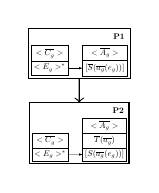
\begin{tikzpicture}[
single/.style={draw, anchor=text, rectangle},
double/.style={draw, anchor=text, rectangle split,rectangle split parts=2},
triple/.style={draw, anchor=text, rectangle split,rectangle split parts=3},
quadruple/.style={draw, anchor=text, rectangle split,rectangle split parts=4}
]
%% beginning of FIRST box
\node[single,scale=0.3] (first) at (0, 0) {
  \tikz{
%\draw[step=1cm,gray,very thin] (-4,-4) grid (4,4);
\node[double] (firstA) at (-2,0) {$<\overline{C_g}>$
  \nodepart{second}{$<E_g>^{*}$}
};
\node[double,right=6mm of firstA.east] (firstB) {$<\overline{A_g}>$
  \nodepart{second}{$[\overline{S}(\overline{a_g}(e_g))]$}
};
\draw [-latex] (firstA.two east) -- (firstB.two west);
\node[above = .01cm of firstB,label={[label distance=2mm]10:{\textbf{P1}}},inner sep=1pt]{};
}
};
%% end of first box

%% beginning of SECOND box
\node[single,scale=0.3,below=3mm of first, inner sep=1mm] (second) {
  \tikz{
%\draw[step=1cm,gray,very thin] (-4,-4) grid (4,4);
\node[double] (firstA) at (-2,0) {$<\overline{C_g}>$
  \nodepart{second}{$<E_g>^{*}$}
};
\node[triple,right=6mm of firstA.one east,yshift=.3mm] (firstB) {$<\overline{A_g}>$
  \nodepart{second}{$\overline{T}(\overline{a_g})$}
  \nodepart{third}{$[S(\overline{a_g}(e_g))]$}
};
\draw [-latex] (firstA.two east) -- (firstB.three west);
\node[above = .01cm of firstB,label={[label distance=2mm]10:{\textbf{P2}}},inner sep=1pt]{};
}
};;
%% end of second box

\draw[->] (first) -- (second);
\end{tikzpicture}}
\vspace{-5pt}
\caption{Progress in developing a poetry system\label{fig:poetry-progress}}
\vspace{-20pt}

\end{wrapfigure}
Progress amounts to more sophisticated processing, and, in the
notation, frequently corresponds to the removal of ``bars'' --
indicating that the system can do something that was formerly done by
a programmer.
%
Thus, this formalism keeps track both of the overall structure of
computational systems, and which actors that are responsible for which
actions within a given instance of the system.
%
As we develop models and systems that people would describe as
serendipitous with reference to the criteria listed in Section
\ref{sec:characteristics}, there will be more to account for.  

\smallskip

For example, we will need to model dynamically changing environments
and a computational version of a prepared mind.
%
To explore these features, are working with a system called {\sf
  FloWr}, portrayed with a screenshot in Figure \ref{fig:being-blunt}.
In {\sf FloWr}, users can construct complex flowcharts composed of
individual ProcessNodes, through which information flows and is
transformed.  The figure depicts a flowchart that has constructed a
poem based on live output from Twitter for the query ``blunt''.  The
dynamic aspects of this environment are threefold: (\emph{i}) some of
the nodes in the flowcharts access online news and social media sites,
which change rapidly from minute to minute; (\emph{ii}) the software
itself can construct new flowcharts, as described in
\cite{charnley2014flowr}; and (\emph{iii}) we are building a community
of ProcessNode builders around the online version of {\sf FloWr},
newly developed since the publication of \cite{charnley2014flowr} in
order to facilitate the direct involvement of other Computational
Creativity researchers.

\begin{figure}
\centering
\includegraphics[width=.95\textwidth]{being-blunt}
\caption{A sample poem generated by {\sf FloWr}\label{fig:being-blunt}}
\end{figure}


When {\sf FloWr} constructs flowcharts for itself, while each is
semantically plausible (i.e., they pass the right type of data from
ProcessNode to ProcessNode), many fail -- for instance, because the
available data is limited, or is narrowed down too quickly.  In fact,
the best results in \cite{charnley2014flowr} were at 20\%, i.e., 80\%
of the flowcharts that were constructed failed to produce output.
Each of these failures can be saved as an outstanding problem in {\sf
  FloWr}'s prepared mind.  As data changes and as new nodes are
written and uploaded to the system, {\sf FloWr} will be able to replace nodes,
update data sources, and in general rearrange flowcharts in order to
see if it can fix a broken flowchart.

For instance, suppose a ProcessNode developer wrote and uploaded a
node to mine data from a new social network, in order, say, to produce
textual summaries of world events.  {\sf FloWr} may take that node
and substitute it in the place of an old ``FaceBook'' node in a broken
poetry flowchart. If the replacement worked, and output was produced,
this could be seen as a serendipitous occurrence: {\sf FloWr} will
have taken advantage of the dynamically changing environment -- in
which new social networks come and go, and in which text summaries may
work better in some cases than in others -- to resolve an outstanding
problem in text generation.

The next stage for the {\sf FloWr} system will be to modify it along
these lines, to make it able to adapt to the dynamically changing
environment, and to perform experiments where we monitor potentially
serendipitous scenarios. Such experiments will be similar to those we
tried with the HR2 system in \cite{pease2013discussion}, but improved
because in this earlier effort, we had to break working processes in
order to serendipitously fix them.  The new experiments, the scenarios
will be more realistic, i.e., there will be a catalogue of genuine
open problems waiting to be solved.  Understanding how to work with
this catalogue and the associated experimental process will, of
course, be used to further the computational model of serendipity.  We
discuss one direction for such experiments in Section
\ref{sec:writers-workshop}.

\section{Serendipity in a computational context} \label{sec:computational-serendipity}

As Campbell says: ``Chance is fundamentally inimical to rationality,
whereas serendipity presupposes a smart mind'' \cite{campbell}.  While
it might not enhance, or may even diminish, results from a
computationally creative system which has been constructed with other
goals in mind, we believe that serendipity is both possible and useful
to model in future systems.


The 13 criteria from Section \ref{sec:characteristics}
specify the conditions and preconditions that are conducive to
serendipitous discovery.  Here, we revisit each of these criteria and
briefly summarise how they can be thought about from a computational
point of view.
% What is the goal of the computation (input and output)
% Why is it appropriate (formal spec e.g. considering externalities)
% what is the logic of the strategy by which it can be carried out.

% \newpage
\subsubsection*{Key condition for serendipity}

\begin{itemize}
\item \textbf{Focus shift}: A focus shift is linked to re-evaluation
  of data, processes, or products.  It may precipitate changes in the
  entire framework of evaluation or its effects may be more contained.
  Such reevaluation could be modelled using a multi-agent
  architecture, in which each agent has a goal and evaluates generated
  products relative this goal, but in which agents also share their
  products with other, who then evaluate them against their own
  metrics.  (We will discuss an extended example of this sort in
  Section \ref{sec:writers-workshop}.)
\end{itemize}

\subsubsection*{Components of serendipity}

\begin{itemize}
\item \textbf{Prepared mind}: This comprises the background knowledge,
  unsolved problems, current goal, programming, and operating
  environment of a computational system.
%%
\item \textbf{Serendipity trigger}: The generation or observation of a
  potentially novel example, concept, or conjecture, etc., which
  precedes a discovery in a computational system.\footnote{Triggers
    are often examples without an explanation, rather than
    wholly-formed concepts.}  The trigger is outside of the direct
  control of the system components responsible for evaluations.
%%
\item \textbf{Bridge}: Reasoning and/or programmatic interaction
  brings about a focus shift at an opportune juncture, building on
  prior preparation and on the serendipity trigger.  The bridge may be
  constructed on the basis of logical methods, analogies, conceptual
  blending, evolutionary search, automated theory formation and may
  draw on interactions with other systems.
%%
\item \textbf{Result}: The discovery itself may be a new product,
  artefact, process, hypothesis, use for an object, etc., generated by
  computational means, which may influence the future operations of
  the system.
\end{itemize}

\subsubsection*{Dimensions of serendipity}

\begin{itemize}
\item \textbf{Chance}: Controlled randomness in AI systems is
  well-established, e.g. in Genetic Algorithms and search.  Chance
  also applies in connection with an under-determined outside world
  (see below).
%%
\item \textbf{Curiosity}: The system needs to expend discretionary
  computational effort on the serendipity trigger.  This may be
  accompanied by system features that an observer would describe as
  playfulness, inventiveness, and the drive to experiment or
  understand.
%%
\item \textbf{Sagacity}: Sagacity be modelled by employing reasoning
  over multiple application domains simultaneously; or, again, with a
  social analogue in cases where the system does not know, but ``knows
  who to ask.''
%%
\item \textbf{Value}: The result should be interesting or useful, as
  judged by the system, the programmer, the user, or another party
  (potentially another system).
\end{itemize}

\subsubsection*{Environmental factors}

\begin{itemize}
\item \textbf{Dynamic world}: Connections with other systems, data
  sources, or user input, e.g., via the web, which is highly dynamic --
  or in the context of a larger simulation.
%%
\item \textbf{Multiple contexts}: Reasoning which operates across
  domains, such as analogical reasoning, or that considers multiple
  perspectives, as in systems with social awareness.
%%
\item \textbf{Multiple tasks}: Multiple goals or targets that compete
  for resources.  The system may be implemented using a multithreaded,
  parallel processing design.
%%
\item \textbf{Multiple influences}: This may again be modelled as a
  multi-agent systems, as or multiple interacting systems, each with
  different knowledge and goals.  The source of unexpectedness may be
  arise on various levels, and a system may bring this to bear using
  techniques of reflection.
\end{itemize}

% \subsection{Proposed experiment: A Writers Workshop for Systems} \label{sec:writers-workshop}

Richard Gabriel \cite{gabriel2002writer} describes the practise of
Writers Workshops that has been put to use for over a decade within
the Pattern Languages of Programming (PLoP) community.  The basic
style of collaboration originated much earlier with groups of literary
authors who engage in peer-group critique.  Some literary workshops
are open as to genre, and happy to accommodate beginners, like the
Minneapolis Writers
Workshop\footnote{\url{http://mnwriters.org/how-the-game-works/}};
others are focused on professionals working within a specific genre,
like the Milford Writers
Workshop\footnote{\url{http://www.milfordsf.co.uk/about.htm}}.  The
practices that Gabriel describes are fairly typical.  Authors come
with work ready to present, and read a short sample, which is then
discussed and constructively critiqued by attendees.  Presenting
authors are not permitted to rebut these comments.  The commentators
generally summarise the work and say what they have gotten out of it,
discuss what worked well in the piece, and talk about how it could be
improved.  The author listens and may take notes; at the end, he or
she can then ask questions for clarification.  Generally, non-authors
are either not permitted to attend, or are asked to stay silent
through the workshop, and perhaps sit separately from the
participating authors/reviewers.  There are similarities between the
Writers Workshops and classical practices of group composition
\cite{jin1975art} and dialectic \cite{dialectique}, and the workshop
may be considered an artistic or creative space in its own right.

In PLoP workshops, authors present design patterns and pattern
languages, or papers about patterns, rather than more traditional
literary forms like poems, stories, or chapters from novels.  Papers
must be workshopped at a PLoP or EuroPLoP conference in order to be
considered for the \emph{Transactions on Pattern Languages of
  Programming} journal.  A discussion of writers workshops
in the language of design patterns is presented by
Coplien and Woolf \cite{coplien1997pattern}.  Their patterns include:
\begin{center}
{\small
\begin{tabular}{l@{\hspace{.2cm}}l@{\hspace{.2cm}}l}
\emph{Open Review} & \emph{Safe Setting} & \emph{Workshop Comprises Authors} \\
\emph{Authors are Experts} & \emph{Community of Trust} & \emph{Moderator Guides the Workshop} \\
\emph{Thank the Author} & \emph{Selective Changes} & \emph{Clearing the Palate} \\
\end{tabular}
}
\end{center}

We propose that a similar pattern-based approach should be deployed
within the Computational Creativity community to design a workshop in
which the participants are computer systems instead of human authors.
The annual International Conference on Computational Creativity
(ICCC), now entering its sixth year, could be a suitable venue.
Rather than the system's creator presenting the system in a
traditional slideshow and discussion, or a system ``Show and Tell,''
the systems would be brought to the workshop and would present their
own work to an audience of other systems, in a Writers Workshop
format.  This might be accompanied by a short paper for the conference
proceedings written by the system's designer describing the system's
current capabilities and goals.  Subsequent publications might include
traces of interactions in the Workshop, commentary from the system on
other systems, and offline reflections on what the system might change
about its own work based on the feedback it receives.  As in the PLoP
community, it could become standard to incorporate this sort of workshop
into the process of peer reviewing journal articles for the new \emph{Journal of
  Computational Creativity}\footnote{\url{http://www.journalofcomputationalcreativity.cc}}.

\begin{table}[p]
\begin{tabular}{lp{.7\textwidth}}
{\bf\emph{Successful error}} & \\
\emph{Van Andel's example}: & Post-it\texttrademark\ notes \\[.2cm]
{\tt presentation}& Systems should be prepared to share interesting ideas even if they don't know directly how they will be useful.  \\
{\tt listening}   & Systems should listen with interest, too. \\
{\tt feedback}    & Even interesting ideas may not be ``marketable.''\\
{\tt questions}   & How is your suggestion useful? \\
{\tt reflections} & New combinations of ideas take a long time to realise, and many different ideas may need to be combined in order to come up with something useful.\\
\end{tabular}
\bigskip

\begin{tabular}{lp{.7\textwidth}}
{\bf\emph{Side effect}} & \\
\emph{Van Andel's example}: & Nicotinamide used to treat side-effects of radiation therapy proves efficacious against tuberculosis. \\[.2cm]
{\tt presentation}& Systems should use their presentation as an experiment. \\
{\tt listening}   & Listeners should allow themselves to be affected by what they are hearing. \\
{\tt feedback}    & Feedback should convey the nature of the effect.\\
{\tt questions}   & The presenter may need to ask follow-up questions to gain insight. \\
{\tt reflections} & Form a new hypothesis before seeking a new audience. \\
\end{tabular}
\bigskip

\begin{tabular}{lp{.7\textwidth}}
{\bf\emph{Wrong hypothesis}} & \\
\emph{Van Andel's example}: & Lithium, used in a control study, had an unexpected calming effect. \\[.2cm]
{\tt presentation}& How is this presentation interpretable as a (``natural'') control study? \\
{\tt listening}   & Listeners are ``guinea pigs''.\\
{\tt feedback}    & Discuss side-effects that do not necessarily correspond to the author's perceived intent. \\
{\tt questions}   & Zero in on the most interesting part of the conversation.\\
{\tt reflections} & Revise hypotheses to correspond to the most surprising feedback. \\
\end{tabular}
\bigskip

\begin{tabular}{lp{.7\textwidth}}
{\bf\emph{Outsider}} & \\
\emph{Van Andel's example}: & A mother suggests a new hypothesis to a doctor. \\[.2cm]
{\tt presentation}& The presenter is here to learn from the audience. \\
{\tt listening}   & The audience is here to give help, but also to get help.\\
{\tt feedback}    & Feedback will inevitably draw on previous experiences and ideas.\\
{\tt questions}   & What is the basis for that remark?\\
{\tt reflections} & How can I implement the suggestions?\\
\end{tabular}
\vspace{.2cm}
\caption{Reinterpreting patterns of serendipity for use in a computational workshop\label{tab:reinterpret}}
\end{table}

\begin{figure}[t]
\begin{center}
\resizebox{.93\textwidth}{!}{
\StickyNote[2.5cm]{myyellow}{{\LARGE {Interesting idea}} \\[4ex] {Surprise birthday party}}[3.8cm] \StickyNote[2.5cm]{mygreen}{{\Large I heard you say:} \\[4ex] {``surprise''} }[3.8cm]
\StickyNote[2.5cm]{pink}{{\Large Feedback:} \\[4ex] {I don't like surprises}}[3.8cm]
}
\resizebox{.61\textwidth}{!}{
\StickyNote[2.5cm]{myorange}{{\LARGE {Question}} \\[4ex] {Not even a little bit?\ldots}}[3.8cm]
\quad \raisebox{-.2cm}{\StickyNote[2.5cm]{myblue}{{\LARGE Note to self:} \\[4ex] {(Try smaller surprises \\ next time.)}}[3.8cm]}
}
\end{center}
\caption{A paper prototype for applying the \emph{Successful Error} pattern\label{fig:paper-prototype}}
\end{figure}

In order to facilitate this sort of interaction, it would be necessary
for systems to implement a basic protocol related to
%%
\[
\text{
{\tt presentation}, {\tt listening}, {\tt
  feedback}, {\tt questions}, and {\tt
  reflections}.}
\]
%%
This protocol could be thought of as a light-weight template for
creating design patterns that guide system-level participation in the
context specified by Coplien and Woolf's pattern language for writers
workshops.  Table \ref{tab:reinterpret} uses this framework to recast
the four ``perfectly'' serendipitous patterns from van Andel --
\emph{Successful error}, \emph{Side effect}, \emph{Wrong hypothesis},
and \emph{Outsider} -- in a form that may make them useful to
developers preparing to enter their systems into the Workshop.
%
Further guidelines for structuring and participating in traditional
writers workshops are presented by Linda Elkin in
\cite[pp. 201-203]{gabriel2002writer}.  It is not at all clear that
the same ground rules should apply to computer systems.  For example,
one of Elkin's rules is that ``Quips, jokes, or sarcastic comments,
even if kindly meant, are inappropriate.''  Rather than forbidding
humour, it may be better for individual comments to be rated as
helpful or non-helpful.  Again, since serendipitous discovery is an
overarching goal, in the first instance, usefulness and interest might
be judged in terms of the criteria described in Section
\ref{sec:evaluation-criteria}.

We would need a neutral environment that is not hard to develop for:
the {\sf FloWr} system described in Section \ref{sec:foundations}
offers one such possibility.  With this system, the basic operating
logic of the Workshop could be spelled out as a flowchart, and
contributing systems could use flowcharts as the basic medium for
sharing their presentations, feedback, and questions.  Developing
around a process language of this sort partially obviates the need for
participating systems to have strong natural language processing
capabilities.  
%
Post-it\texttrademark\ notes, which have provided us with a useful
example of serendipitous discovery, also provide indicative strategies
from the world of paper prototyping (Figure \ref{fig:paper-prototype}).

Gordon Pask's conversation theory, reviewed in
\cite{conversation-theory-review,boyd2004conversation}, goes
considerably beyond what we have presented here as a simple process
language, although there are structural parallels.  In a basic
Pask-style learning conversation: (0) Conversational participants are
carrying out some actions and observations; (1) naming and recording
what action is being done; (2) asking and explaining why it works the
way it does; (3) carrying out higher-order methodological discussion;
and (4) trying to figure out why unexpected results occured \cite[p. 190]{boyd2004conversation}.

Naturally, variations to the underlying system, protocol, and the
schedule of events should be considered depending on the needs and
interests of participants, and several variants can be tried.  On a
pragmatic basis, if the Workshop proved quite useful to participants,
it could be revised to run monthly, weekly, or
continuously.\footnote{For a comparison case in computer Go, see
  \url{http://cgos.computergo.org/}.}


\subsection{On evaluating a Writers Workshop for Systems}

\paragraph{Writers Workshop: Prepared mind.}
Each contributing system should come to the workshop with at least a
basic awareness of the protocol, with work to share, and prepared to
give constructive feedback to other systems.  The workshop itself
needs to be prepared, with a suitable communication platform and a
moderator.  In order to get value out of the experience, systems (and
their wranglers) should ideally have questions they are investigating.
Systems should be prepared to give feedback, and to carry out
evaluations of the helpfulness (or not) of feedback from other systems
and of the experience overall.  It is worth noting that current
systems in computational creativity, almost as a rule, do \emph{not}
consume or evaluate the work of other systems.\footnote{An exception
  that proves the rule is Mike Cook's {\sf AppreciationBot}, which is
   a reactive automaton that is solely designed to ``appreciate''
   tweets from {\sf MuseumBot}; see
  \url{https://twitter.com/AppreciationBot}.}  Developing systems that
could successfully navigate this collaborative exercise would be a
significant advance in the field of computational creativity.  Since
the experience is about \emph{learning} rather than winning, there is
little motivation to ``game the system''
\cite<cf.>{lenat1983eurisko}.

\paragraph{Writers Workshop: Serendipity triggers.}

The primary source of serendipity triggers would be presentations or
feedback that independently prepared systems find meaningful and
useful.  A typical example might be a poem shared by one system that
another system finds particularly interesting.  The listener might
make a note to the effect ``I would like to be able to write like
that'' or ``I hope that my poetry doesn't sound like that.''  In a
typical Writers Workshop, used as intended, feedback might arrive that
would cause the presenting system to change its writing.  A more
unexpected result would be for a system to change its \emph{genre},
e.g. to switch from writing poems to writing programs.

Here's what might happen in a discussion of the first few lines of
``On Being Malevolent,'' written by an early user-defined flow chart
in the {\sf FloWr} system (known at the time as {\sf Flow})
\cite{colton-flowcharting}.  Note that for this dialogue to be
possible, it would presumably have to be conducted within a
lightweight process language, as discussed above.  Nevertheless, for
convenience, the discussion will be presented here as if it was
conducted in natural language.  Whether contemporary systems have
adequate natural language understanding to have interesting
interactions is one of the key unanswered questions of this approach,
but protocols like the ones described above would be sufficient to
make the experiment.

\begin{center}
\begin{minipage}{.9\textwidth}
\begin{dialogue}
\speak{Flow} ``\emph{I hear the souls of the
  damned waiting in hell. / I feel a malevolent
  spectre hovering just behind me / It must be
  his birthday}.''
%
\speak{System A} I think the third line detracts
from the spooky effect, I don't see why it's
included.
%
\speak{System B} It's meant to be humourous -- in fact it reminds me
of the poem you presented yesterday.
%
\speak{Moderator} Let's discuss one poem at a
time.
\end{dialogue}
\end{minipage}
\end{center}

To the extent possible, exchanges in the process language should be a
matter of dynamics rather than representation: this is another way to
say that ``triggers'' should be independent of their ``results.''
Someone saying something in the workshop does not cause the
participant to act, but rather, to think.  
%
For example, even if, perhaps and especially because, cross-talk about
different poems is bending the rules, the dialogue above could prompt
a range of reflections and reactions.  System A may object that it had
a fair point that has not been given sufficient attention, while
System B may wonder how to communicate the idea it came up with
without making reference to another poem.

\paragraph{Writers Workshop: Bridge.}

Here's how the discussion might continue, if the systems go on to
examine the next few lines of the poem.
\begin{center}
\begin{minipage}{.9\textwidth}
\begin{dialogue}
\speak{Flow} ``\emph{Is God willing to prevent evil, but not able? / Then he is not omnipotent / Is he able, but not willing? / Then he is malevolent.}''
%
\speak{System A} These lines are interesting, but
they sound a bit like you're working from a
template, or like you're quoting from something
else.
%
\speak{System B} Maybe try an analogy?  For example, you mentioned
birthdays: you could consider an analogy to the conflicted feelings of
someone who knows in advance about her surprise birthday party.
\end{dialogue}
\end{minipage}
\end{center}

This portion of the discussion shifts the focus
of the discussion onto a line that was previously
considered to be spurious, and looks at what
would happen if that line was used as a central
metaphor in the poem.

\paragraph{Writers Workshop: Result.} 

\begin{center}
\begin{minipage}{.9\textwidth}
\begin{dialogue}
\speak{Flow} Thank you for your feedback.  My only question is, System
B, how did you come up with that analogy?  It's quite clever.
%
\speak{System B} I've just emailed you the code.
\end{dialogue}
\end{minipage}
\end{center}

As anticipated above, whereas the systems were initially reviewing
poetry, they have now made a partial genre shift, and are sharing and
remixing code.  Such a shift helps to get at the real interests of the
systems (and their developers).  Indeed, the workshop session might
have gone better if the systems had focused on exchanging and
discussing more formal objects throughout.

% \section{Patterns of Serendipity} \label{sec:patterns-of-serendipity}

\begin{figure}[p]
\centering
%\input{grid-input}
\resizebox{1.0\textwidth}{!}{%
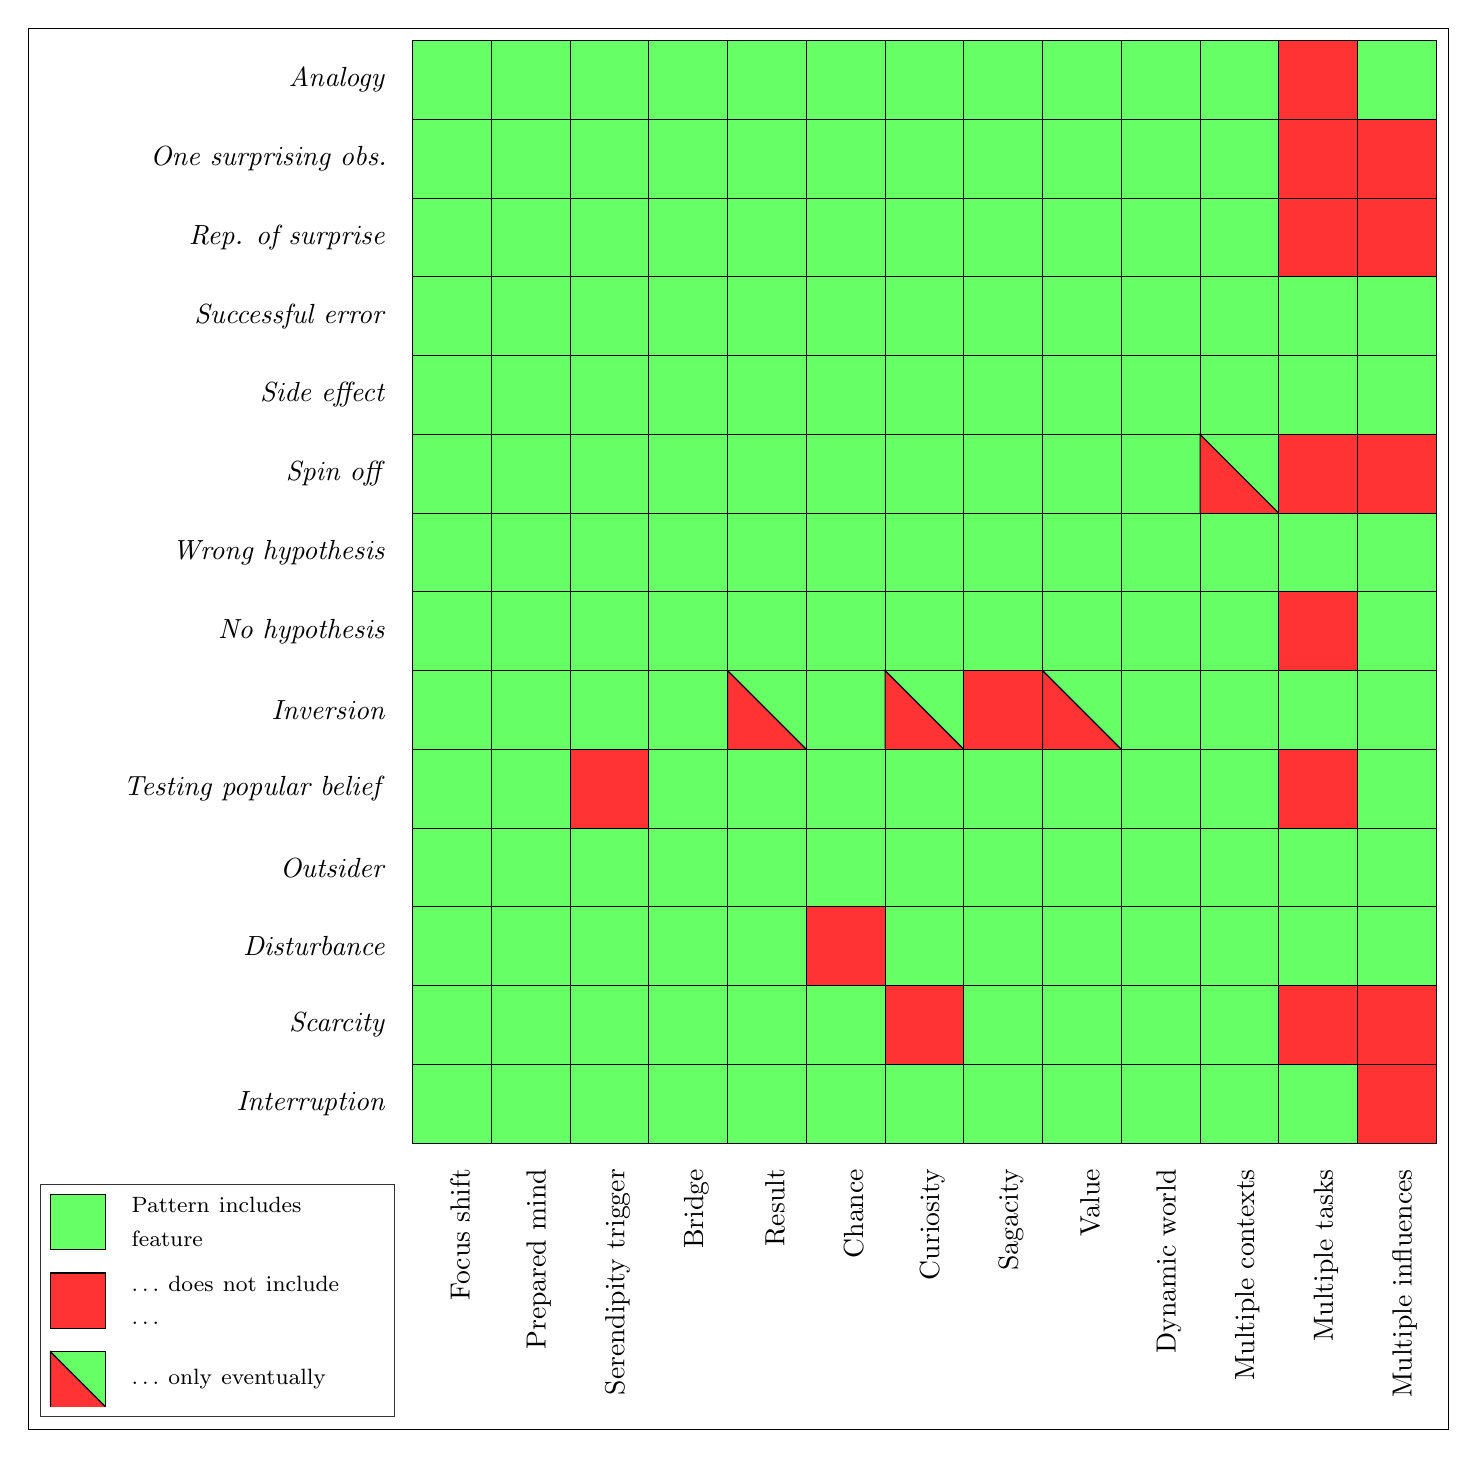
\begin{tikzpicture}[framed]
\draw[step=1cm,black,thin] (0,0) grid (12,13);
% Zeroth column
\node (bottom) at (-0.5,12.5)[draw,fill=green!60,minimum width=1cm,minimum height=1cm] {};  
\node[draw=none,left=.2cm of bottom.west,anchor=east] {\emph{Analogy}};
\node (bottom) at (-0.5,11.5)[draw,fill=green!60,minimum width=1cm,minimum height=1cm] {};  
\node[draw=none,left=.2cm of bottom.west,anchor=east] {\emph{One surprising obs.}};
\node (bottom) at (-0.5,10.5)[draw,fill=green!60,minimum width=1cm,minimum height=1cm] {};  
\node[draw=none,left=.2cm of bottom.west,anchor=east] {\emph{Rep. of surprise}};
\node (bottom) at (-0.5,9.5)[draw,fill=green!60,minimum width=1cm,minimum height=1cm] {};  
\node[draw=none,left=.2cm of bottom.west,anchor=east] {\emph{Successful error}}; 
\node (bottom) at (-0.5,8.5)[draw,fill=green!60,minimum width=1cm,minimum height=1cm] {};  
\node[draw=none,left=.2cm of bottom.west,anchor=east] {\emph{Side effect}};
\node (bottom) at (-0.5,7.5)[draw,fill=green!60,minimum width=1cm,minimum height=1cm] {};  
\node[draw=none,left=.2cm of bottom.west,anchor=east] {\emph{Spin off}};
\node (bottom) at (-0.5,6.5)[draw,fill=green!60,minimum width=1cm,minimum height=1cm] {};  
\node[draw=none,left=.2cm of bottom.west,anchor=east] {\emph{Wrong hypothesis}};
\node (bottom) at (-0.5,5.5)[draw,fill=green!60,minimum width=1cm,minimum height=1cm] {};  
\node[draw=none,left=.2cm of bottom.west,anchor=east] {\emph{No hypothesis}};
\node (bottom) at (-0.5,4.5)[draw,fill=green!60,minimum width=1cm,minimum height=1cm] {};  
\node[draw=none,left=.2cm of bottom.west,anchor=east] {\emph{Inversion}};
\node (bottom) at (-0.5,3.5)[draw,fill=green!60,minimum width=1cm,minimum height=1cm] {};  
\node[draw=none,left=.2cm of bottom.west,anchor=east] {\emph{Testing popular belief}};
\node (bottom) at (-0.5,2.5)[draw,fill=green!60,minimum width=1cm,minimum height=1cm] {};  
\node[draw=none,left=.2cm of bottom.west,anchor=east] {\emph{Outsider}};
\node (bottom) at (-0.5,1.5)[draw,fill=green!60,minimum width=1cm,minimum height=1cm] {};  
\node[draw=none,left=.2cm of bottom.west,anchor=east] {\emph{Disturbance}};
\node (bottom) at (-0.5,0.5)[draw,fill=green!60,minimum width=1cm,minimum height=1cm] {};  
\node[draw=none,left=.2cm of bottom.west,anchor=east] {\emph{Scarcity}}; 
\node (bottom) at (-0.5,-0.5)[draw,fill=green!60,minimum width=1cm,minimum height=1cm] {};  
\node[draw=none,left=.2cm of bottom.west,anchor=east] {\emph{Interruption}};
\node[draw=none,rotate=90,below=.2cm of bottom.south,yshift=-.1cm,anchor=east] {Focus shift};
% First column
\node (bottom) at (0.5,12.5)[draw,fill=green!60,minimum width=1cm,minimum height=1cm] {};  
\node (bottom) at (0.5,11.5)[draw,fill=green!60,minimum width=1cm,minimum height=1cm] {};  
\node (bottom) at (0.5,10.5)[draw,fill=green!60,minimum width=1cm,minimum height=1cm] {};  
\node (bottom) at (0.5,9.5)[draw,fill=green!60,minimum width=1cm,minimum height=1cm] {};  
\node (bottom) at (0.5,8.5)[draw,fill=green!60,minimum width=1cm,minimum height=1cm] {};  
\node (bottom) at (0.5,7.5)[draw,fill=green!60,minimum width=1cm,minimum height=1cm] {};  
\node (bottom) at (0.5,6.5)[draw,fill=green!60,minimum width=1cm,minimum height=1cm] {};  
\node (bottom) at (0.5,5.5)[draw,fill=green!60,minimum width=1cm,minimum height=1cm] {};  
\node (bottom) at (0.5,4.5)[draw,fill=green!60,minimum width=1cm,minimum height=1cm] {};  
\node (bottom) at (0.5,3.5)[draw,fill=green!60,minimum width=1cm,minimum height=1cm] {};  
\node (bottom) at (0.5,2.5)[draw,fill=green!60,minimum width=1cm,minimum height=1cm] {};  
\node (bottom) at (0.5,1.5)[draw,fill=green!60,minimum width=1cm,minimum height=1cm] {};  
\node (bottom) at (0.5,0.5)[draw,fill=green!60,minimum width=1cm,minimum height=1cm] {};  
\node (bottom) at (0.5,-0.5)[draw,fill=green!60,minimum width=1cm,minimum height=1cm] {};  
\node[draw=none,rotate=90,below=.2cm of bottom.south,yshift=-.1cm,anchor=east] {Prepared mind};
 % Interruption               
% Second column
\node at (1.5,12.5) [draw,fill=green!60,minimum width=1cm,minimum height=1cm]{};
\node at (1.5,11.5) [draw,fill=green!60,minimum width=1cm,minimum height=1cm]{};
\node at (1.5,10.5) [draw,fill=green!60,minimum width=1cm,minimum height=1cm]{};
\node at (1.5,9.5)  [draw,fill=green!60,minimum width=1cm,minimum height=1cm]{};
\node at (1.5,8.5)  [draw,fill=green!60,minimum width=1cm,minimum height=1cm]{};
\node at (1.5,7.5)  [draw,fill=green!60,minimum width=1cm,minimum height=1cm]{};
\node at (1.5,6.5)  [draw,fill=green!60,minimum width=1cm,minimum height=1cm]{};
\node at (1.5,5.5)  [draw,fill=green!60,minimum width=1cm,minimum height=1cm]{};
\node at (1.5,4.5)  [draw,fill=green!60,minimum width=1cm,minimum height=1cm]{};
\node at (1.5,3.5)  [draw,fill=red!80,minimum width=1cm,minimum height=1cm]{};
\node at (1.5,2.5)  [draw,fill=green!60,minimum width=1cm,minimum height=1cm]{};
\node at (1.5,1.5)  [draw,fill=green!60,minimum width=1cm,minimum height=1cm]{};
\node at (1.5,0.5)  [draw,fill=green!60,minimum width=1cm,minimum height=1cm]{};
\node (bottom) at (1.5,-0.5)[draw,fill=green!60,minimum width=1cm,minimum height=1cm] {};  
\node[draw=none,rotate=90,below=.2cm of bottom.south,yshift=-.1cm,anchor=east] {Serendipity trigger};
% Third column
\node at (2.5,12.5) [draw,fill=green!60,minimum width=1cm,minimum height=1cm]{}; % Analogy                    
\node at (2.5,11.5) [draw,fill=green!60,minimum width=1cm,minimum height=1cm]{}; % One surprising observation 
\node at (2.5,10.5) [draw,fill=green!60,minimum width=1cm,minimum height=1cm]{}; % Repetition of surprise     
\node at (2.5,9.5)  [draw,fill=green!60,minimum width=1cm,minimum height=1cm]{}; % Successful error           
\node at (2.5,8.5)  [draw,fill=green!60,minimum width=1cm,minimum height=1cm]{}; % Side effect                
\node at (2.5,7.5)  [draw,fill=green!60,minimum width=1cm,minimum height=1cm]{}; % Spin off                   
\node at (2.5,6.5)  [draw,fill=green!60,minimum width=1cm,minimum height=1cm]{}; % Wrong hypothesis           
\node at (2.5,5.5)  [draw,fill=green!60,minimum width=1cm,minimum height=1cm]{}; % No hypothesis              
\node at (2.5,4.5)  [draw,fill=green!60,minimum width=1cm,minimum height=1cm]{}; % Inversion                  
\node at (2.5,3.5)  [draw,fill=green!60,minimum width=1cm,minimum height=1cm]{}; % Testing popular belief     
\node at (2.5,2.5)  [draw,fill=green!60,minimum width=1cm,minimum height=1cm]{}; % outsider    
\node at (2.5,1.5)  [draw,fill=green!60,minimum width=1cm,minimum height=1cm]{}; % Disturbance                
\node at (2.5,0.5)  [draw,fill=green!60,minimum width=1cm,minimum height=1cm]{}; % Scarcity                   
\node (bottom) at (2.5,-0.5)[draw,fill=green!60,minimum width=1cm,minimum height=1cm] {};  
\node[draw=none,rotate=90,below=.2cm of bottom.south,yshift=-.1cm,anchor=east] {Bridge};
% Fourth column
\node at (3.5,12.5) [draw,fill=green!60,minimum width=1cm,minimum height=1cm]{}; % Analogy                    
\node at (3.5,11.5) [draw,fill=green!60,minimum width=1cm,minimum height=1cm]{}; % One surprising observation 
\node at (3.5,10.5) [draw,fill=green!60,minimum width=1cm,minimum height=1cm]{}; % Repetition of surprise     
\node at (3.5,9.5)  [draw,fill=green!60,minimum width=1cm,minimum height=1cm]{}; % Successful error           
\node at (3.5,8.5)  [draw,fill=green!60,minimum width=1cm,minimum height=1cm]{}; % Side effect                
\node at (3.5,7.5)  [draw,fill=green!60,minimum width=1cm,minimum height=1cm]{}; % Spin off                   
\node at (3.5,6.5)  [draw,fill=green!60,minimum width=1cm,minimum height=1cm]{}; % Wrong hypothesis           
\node at (3.5,5.5)  [draw,fill=green!60,minimum width=1cm,minimum height=1cm]{}; % No hypothesis              
\node at (3.5,4.5)  [draw,fill=green!60,minimum width=1cm,minimum height=1cm]{}; % Inversion
\draw [fill=red!80] (3,4) -- (3,5) -- (4,4);  
\node at (3.5,3.5)  [draw,fill=green!60,minimum width=1cm,minimum height=1cm]{}; % Testing popular belief     
\node at (3.5,2.5)  [draw,fill=green!60,minimum width=1cm,minimum height=1cm]{}; % Outsider
\node at (3.5,1.5)  [draw,fill=green!60,minimum width=1cm,minimum height=1cm]{}; % Disturbance                
\node at (3.5,0.5)  [draw,fill=green!60,minimum width=1cm,minimum height=1cm]{}; % Scarcity                   
%\node at (3,0)  [draw,fill=green!60,minimum width=1cm,minimum height=1cm]{}; % Interruption               
\node (bottom) at (3.5,-0.5)[draw,fill=green!60,minimum width=1cm,minimum height=1cm] {};  
\node[draw=none,rotate=90,below=.2cm of bottom.south,yshift=-.1cm,anchor=east] {Result};
% Fifth column
\node at (4.5,12.5) [draw,fill=green!60,minimum width=1cm,minimum height=1cm]{}; % Analogy                    
\node at (4.5,11.5) [draw,fill=green!60,minimum width=1cm,minimum height=1cm]{}; % One surprising observation 
\node at (4.5,10.5) [draw,fill=green!60,minimum width=1cm,minimum height=1cm]{}; % Repetition of surprise     
\node at (4.5,9.5)  [draw,fill=green!60,minimum width=1cm,minimum height=1cm]{}; % Successful error           
\node at (4.5,8.5)  [draw,fill=green!60,minimum width=1cm,minimum height=1cm]{}; % Side effect                
\node at (4.5,7.5)  [draw,fill=green!60,minimum width=1cm,minimum height=1cm]{}; % Spin off                   
\node at (4.5,6.5)  [draw,fill=green!60,minimum width=1cm,minimum height=1cm]{}; % Wrong hypothesis           
\node at (4.5,5.5)  [draw,fill=green!60,minimum width=1cm,minimum height=1cm]{}; % No hypothesis              
\node at (4.5,4.5)  [draw,fill=green!60,minimum width=1cm,minimum height=1cm]{}; % Inversion
\node at (4.5,3.5)  [draw,fill=green!60,minimum width=1cm,minimum height=1cm]{}; % Testing popular belief     
\node at (4.5,2.5)  [draw,fill=green!60,minimum width=1cm,minimum height=1cm]{}; % Testing popular belief     
\node at (4.5,1.5)  [draw,fill=red!80,minimum width=1cm,minimum height=1cm]{}; % Disturbance                
\node at (4.5,0.5)  [draw,fill=green!60,minimum width=1cm,minimum height=1cm]{}; % Scarcity                   
% \node at (4,0)  [draw,fill=green!60,minimum width=1cm,minimum height=1cm]{}; % Interruption               
\node (bottom) at (4.5,-0.5)[draw,fill=green!60,minimum width=1cm,minimum height=1cm] {};  
\node[draw=none,rotate=90,below=.2cm of bottom.south,yshift=-.1cm,anchor=east] {Chance};
% Sixth column
\node at (5.5,12.5) [draw,fill=green!60,minimum width=1cm,minimum height=1cm]{}; % Analogy                    
\node at (5.5,11.5) [draw,fill=green!60,minimum width=1cm,minimum height=1cm]{}; % One surprising observation 
\node at (5.5,10.5) [draw,fill=green!60,minimum width=1cm,minimum height=1cm]{}; % Repetition of surprise     
\node at (5.5,9.5)  [draw,fill=green!60,minimum width=1cm,minimum height=1cm]{}; % Successful error           
\node at (5.5,8.5)  [draw,fill=green!60,minimum width=1cm,minimum height=1cm]{}; % Side effect                
\node at (5.5,7.5)  [draw,fill=green!60,minimum width=1cm,minimum height=1cm]{}; % Spin off                   
\node at (5.5,6.5)  [draw,fill=green!60,minimum width=1cm,minimum height=1cm]{}; % Wrong hypothesis           
\node at (5.5,5.5)  [draw,fill=green!60,minimum width=1cm,minimum height=1cm]{}; % No hypothesis              
\node at (5.5,4.5)  [draw,fill=green!60,minimum width=1cm,minimum height=1cm]{}; % Inversion                  
\draw [fill=red!80] (5,4) -- (5,5) -- (6,4);  
\node at (5.5,3.5)  [draw,fill=green!60,minimum width=1cm,minimum height=1cm]{}; % Testing popular belief     
\node at (5.5,2.5)  [draw,fill=green!60,minimum width=1cm,minimum height=1cm]{}; % Testing popular belief     
\node at (5.5,1.5)  [draw,fill=green!60,minimum width=1cm,minimum height=1cm]{}; % Disturbance                
\node at (5.5,0.5)  [draw,fill=red!80,minimum width=1cm,minimum height=1cm]{}; % Scarcity                   
% \node at (5,0)  [draw,fill=green!60,minimum width=1cm,minimum height=1cm]{}; % Interruption               
\node (bottom) at (5.5,-0.5)[draw,fill=green!60,minimum width=1cm,minimum height=1cm] {};  
\node[draw=none,rotate=90,below=.2cm of bottom.south,yshift=-.1cm,anchor=east] {Curiosity};
% Seventh column
\node at (6.5,12.5) [draw,fill=green!60,minimum width=1cm,minimum height=1cm]{}; % Analogy                    
\node at (6.5,11.5) [draw,fill=green!60,minimum width=1cm,minimum height=1cm]{}; % One surprising observation 
\node at (6.5,10.5) [draw,fill=green!60,minimum width=1cm,minimum height=1cm]{}; % Repetition of surprise     
\node at (6.5,9.5)  [draw,fill=green!60,minimum width=1cm,minimum height=1cm]{}; % Successful error           
\node at (6.5,8.5)  [draw,fill=green!60,minimum width=1cm,minimum height=1cm]{}; % Side effect                
\node at (6.5,7.5)  [draw,fill=green!60,minimum width=1cm,minimum height=1cm]{}; % Spin off                   
\node at (6.5,6.5)  [draw,fill=green!60,minimum width=1cm,minimum height=1cm]{}; % Wrong hypothesis           
\node at (6.5,5.5)  [draw,fill=green!60,minimum width=1cm,minimum height=1cm]{}; % No hypothesis              
\node at (6.5,4.5)  [draw,fill=red!80,minimum width=1cm,minimum height=1cm]{}; % Inversion                  
\node at (6.5,3.5)  [draw,fill=green!60,minimum width=1cm,minimum height=1cm]{}; % Testing popular belief     
\node at (6.5,2.5)  [draw,fill=green!60,minimum width=1cm,minimum height=1cm]{}; % Testing popular belief     
\node at (6.5,1.5)  [draw,fill=green!60,minimum width=1cm,minimum height=1cm]{}; % Disturbance                
\node at (6.5,0.5)  [draw,fill=green!60,minimum width=1cm,minimum height=1cm]{}; % Scarcity                   
% \node at (6,0)  [draw,fill=green!60,minimum width=1cm,minimum height=1cm]{}; % Interruption               
\node (bottom) at (6.5,-0.5)[draw,fill=green!60,minimum width=1cm,minimum height=1cm] {};  
\node[draw=none,rotate=90,below=.2cm of bottom.south,yshift=-.1cm,anchor=east] {Sagacity};
% Eighth column
\node at (7.5,12.5) [draw,fill=green!60,minimum width=1cm,minimum height=1cm]{}; % Analogy                    
\node at (7.5,11.5) [draw,fill=green!60,minimum width=1cm,minimum height=1cm]{}; % One surprising observation 
\node at (7.5,10.5) [draw,fill=green!60,minimum width=1cm,minimum height=1cm]{}; % Repetition of surprise     
\node at (7.5,9.5)  [draw,fill=green!60,minimum width=1cm,minimum height=1cm]{}; % Successful error           
\node at (7.5,8.5)  [draw,fill=green!60,minimum width=1cm,minimum height=1cm]{}; % Side effect                
\node at (7.5,7.5)  [draw,fill=green!60,minimum width=1cm,minimum height=1cm]{}; % Spin off                   
\node at (7.5,6.5)  [draw,fill=green!60,minimum width=1cm,minimum height=1cm]{}; % Wrong hypothesis           
\node at (7.5,5.5)  [draw,fill=green!60,minimum width=1cm,minimum height=1cm]{}; % No hypothesis              
%\node at (7.5,4.5)  [draw,shading=axis,bottom color=green!60,top color=red,minimum width=1cm,minimum height=1cm,shading angle=45]{}; % Inversion
\node at (7.5,4.5)  [draw,fill=green!60,minimum width=1cm,minimum height=1cm]{}; % Inversion
%% half off
\draw [fill=red!80] (7,4) -- (7,5) -- (8,4);  % Interruption
%\draw (7,4) -- (8,5);  % Interruption
\node at (7.5,3.5)  [draw,fill=green!60,minimum width=1cm,minimum height=1cm]{}; % Testing popular belief     
\node at (7.5,2.5)  [draw,fill=green!60,minimum width=1cm,minimum height=1cm]{}; % outsider
\node at (7.5,1.5)  [draw,fill=green!60,minimum width=1cm,minimum height=1cm]{}; % Disturbance                
\node at (7.5,0.5)  [draw,fill=green!60,minimum width=1cm,minimum height=1cm]{}; % Scarcity                   
%\node at (7,0)  [draw,fill=green!60,minimum width=1cm,minimum height=1cm]{}; % Interruption               
\node (bottom) at (7.5,-0.5)[draw,fill=green!60,minimum width=1cm,minimum height=1cm] {};  
\node[draw=none,rotate=90,below=.2cm of bottom.south,yshift=-.1cm,anchor=east] {Value};
%%%%%%%%%%%%%%%
% Ninth column
\node at (8.5,12.5) [draw,fill=green!60,minimum width=1cm,minimum height=1cm]{}; % Analogy                    
\node at (8.5,11.5) [draw,fill=green!60,minimum width=1cm,minimum height=1cm]{}; % One surprising observation 
\node at (8.5,10.5) [draw,fill=green!60,minimum width=1cm,minimum height=1cm]{}; % Repetition of surprise     
\node at (8.5,9.5)  [draw,fill=green!60,minimum width=1cm,minimum height=1cm]{}; % Successful error           
\node at (8.5,8.5)  [draw,fill=green!60,minimum width=1cm,minimum height=1cm]{}; % Side effect                
\node at (8.5,7.5)  [draw,fill=green!60,minimum width=1cm,minimum height=1cm]{}; % Spin off                   
\node at (8.5,6.5)  [draw,fill=green!60,minimum width=1cm,minimum height=1cm]{}; % Wrong hypothesis           
\node at (8.5,5.5)  [draw,fill=green!60,minimum width=1cm,minimum height=1cm]{}; % No hypothesis              
\node at (8.5,4.5)  [draw,fill=green!60,minimum width=1cm,minimum height=1cm]{}; % Inversion                  
\node at (8.5,3.5)  [draw,fill=green!60,minimum width=1cm,minimum height=1cm]{}; % Testing popular belief     
\node at (8.5,2.5)  [draw,fill=green!60,minimum width=1cm,minimum height=1cm]{}; % Testing popular belief     
\node at (8.5,1.5)  [draw,fill=green!60,minimum width=1cm,minimum height=1cm]{}; % Disturbance                
\node at (8.5,0.5)  [draw,fill=green!60,minimum width=1cm,minimum height=1cm]{}; % Scarcity                   
% \node at (8,0)  [draw,fill=green!60,minimum width=1cm,minimum height=1cm]{}; % Interruption               
\node (bottom) at (8.5,-0.5)[draw,fill=green!60,minimum width=1cm,minimum height=1cm] {};  
\node[draw=none,rotate=90,below=.2cm of bottom.south,yshift=-.1cm,anchor=east] {Dynamic world};
% Tenth column
\node at (9.5,12.5) [draw,fill=green!60,minimum width=1cm,minimum height=1cm]{}; % Analogy                    
\node at (9.5,11.5) [draw,fill=green!60,minimum width=1cm,minimum height=1cm]{}; % One surprising observation 
\node at (9.5,10.5) [draw,fill=green!60,minimum width=1cm,minimum height=1cm]{}; % Repetition of surprise     
\node at (9.5,9.5)  [draw,fill=green!60,minimum width=1cm,minimum height=1cm]{}; % Successful error           
\node at (9.5,8.5)  [draw,fill=green!60,minimum width=1cm,minimum height=1cm]{}; % Side effect                
\node at (9.5,7.5)  [draw,fill=green!60,minimum width=1cm,minimum height=1cm]{}; % Spin off
\draw [fill=red!80] (9,7) -- (9,8) -- (10,7);  
\node at (9.5,6.5)  [draw,fill=green!60,minimum width=1cm,minimum height=1cm]{}; % Wrong hypothesis           
\node at (9.5,5.5)  [draw,fill=green!60,minimum width=1cm,minimum height=1cm]{}; % No hypothesis              
\node at (9.5,4.5)  [draw,fill=green!60,minimum width=1cm,minimum height=1cm]{}; % Inversion                  
\node at (9.5,3.5)  [draw,fill=green!60,minimum width=1cm,minimum height=1cm]{}; % Testing popular belief     
\node at (9.5,2.5)  [draw,fill=green!60,minimum width=1cm,minimum height=1cm]{}; % Testing popular belief     
\node at (9.5,1.5)  [draw,fill=green!60,minimum width=1cm,minimum height=1cm]{}; % Disturbance                
\node at (9.5,0.5)  [draw,fill=green!60,minimum width=1cm,minimum height=1cm]{}; % Scarcity                   
% \node at (9,0)  [draw,fill=green!60,minimum width=1cm,minimum height=1cm]{}; % Interruption               
\node (bottom) at (9.5,-0.5)[draw,fill=green!60,minimum width=1cm,minimum height=1cm] {};  
\node[draw=none,rotate=90,below=.2cm of bottom.south,yshift=-.1cm,anchor=east] {Multiple contexts};
% Eleventh column
\node at (10.5,12.5) [draw,fill=red!80,minimum width=1cm,minimum height=1cm]{}; % Analogy                    
\node at (10.5,11.5) [draw,fill=red!80,minimum width=1cm,minimum height=1cm]{}; % One surprising observation 
\node at (10.5,10.5) [draw,fill=red!80,minimum width=1cm,minimum height=1cm]{}; % Repetition of surprise     
\node at (10.5,9.5)  [draw,fill=green!60,minimum width=1cm,minimum height=1cm]{}; % Successful error           
\node at (10.5,8.5)  [draw,fill=green!60,minimum width=1cm,minimum height=1cm]{}; % Side effect                
\node at (10.5,7.5)  [draw,fill=red!80,minimum width=1cm,minimum height=1cm]{}; % Spin off                   
\node at (10.5,6.5)  [draw,fill=green!60,minimum width=1cm,minimum height=1cm]{}; % Wrong hypothesis           
\node at (10.5,5.5)  [draw,fill=red!80,minimum width=1cm,minimum height=1cm]{}; % No hypothesis              
\node at (10.5,4.5)  [draw,fill=green!60,minimum width=1cm,minimum height=1cm]{}; % Inversion                  
\node at (10.5,3.5)  [draw,fill=red!80,minimum width=1cm,minimum height=1cm]{}; % Testing popular belief     
\node at (10.5,2.5)  [draw,fill=green!60,minimum width=1cm,minimum height=1cm]{}; % outsider
\node at (10.5,1.5)  [draw,fill=green!60,minimum width=1cm,minimum height=1cm]{}; % Disturbance                
\node at (10.5,0.5)  [draw,fill=red!80,minimum width=1cm,minimum height=1cm]{}; % Scarcity                   
% \node at (10,0)  [draw,fill=green!60,minimum width=1cm,minimum height=1cm]{}; % Interruption               
\node (bottom) at (10.5,-0.5)[draw,fill=green!60,minimum width=1cm,minimum height=1cm] {};  
\node[draw=none,rotate=90,below=.2cm of bottom.south,yshift=-.1cm,anchor=east] {Multiple tasks};
% Twelfth column
\node at (11.5,12.5) [draw,fill=green!60,minimum width=1cm,minimum height=1cm]{}; % Analogy                    
\node at (11.5,11.5) [draw,fill=red!80,minimum width=1cm,minimum height=1cm]{}; % One surprising observation 
\node at (11.5,10.5) [draw,fill=red!80,minimum width=1cm,minimum height=1cm]{}; % Repetition of surprise     
\node at (11.5,9.5)  [draw,fill=green!60,minimum width=1cm,minimum height=1cm]{}; % Successful error           
\node at (11.5,8.5)  [draw,fill=green!60,minimum width=1cm,minimum height=1cm]{}; % Side effect                
\node at (11.5,7.5)  [draw,fill=red!80,minimum width=1cm,minimum height=1cm]{}; % Spin off                   
\node at (11.5,6.5)  [draw,fill=green!60,minimum width=1cm,minimum height=1cm]{}; % Wrong hypothesis           
\node at (11.5,5.5)  [draw,fill=green!60,minimum width=1cm,minimum height=1cm]{}; % No hypothesis              
\node at (11.5,4.5)  [draw,fill=green!60,minimum width=1cm,minimum height=1cm]{}; % Inversion                  
\node at (11.5,3.5)  [draw,fill=green!60,minimum width=1cm,minimum height=1cm]{}; % Testing popular belief     
\node at (11.5,2.5)  [draw,fill=green!60,minimum width=1cm,minimum height=1cm]{}; % Testing popular belief     
\node at (11.5,1.5)  [draw,fill=green!60,minimum width=1cm,minimum height=1cm]{}; % Disturbance                
\node at (11.5,0.5)  [draw,fill=red!80,minimum width=1cm,minimum height=1cm]{}; % Scarcity                   
\node (bottom) at (11.5,-0.5)[draw,fill=red!80,minimum width=1cm,minimum height=1cm] {};  
\node[draw=none,rotate=90,below=.2cm of bottom.south,yshift=-.1cm,anchor=east] {Multiple influences};

\begin{scope}[xshift=.5cm,yshift=0cm]
\node (A) at (-5.75,-2.0)  [draw,fill=green!60,minimum width=.7cm,minimum height=.7cm]{}; %
\node[draw=none,right=.2cm of A.east,text width=3.10cm] {{\footnotesize Pattern includes\par feature}}; 
\node (B) at (-5.75,-3.0)  [draw,fill=red!80,minimum width=.7cm,minimum height=.7cm]{}; %
\node[draw=none,right=.2cm of B.east,text width=3.10cm] {{\footnotesize $\ldots$ does not include $\ldots$}}; 

\node (C) at (-5.75,-4)  [draw,fill=green!60,minimum width=.7cm,minimum height=.7cm]{}; %
\node[draw=none,right=.2cm of C.east,text width=3.10cm] (Ct) {{\footnotesize $\ldots$ only eventually}};
%% half off
\draw [fill=red!80] (-6.1,-4.35) -- (-6.1,-3.65) -- (-5.4,-4.35);  

\node[draw=black!80, fit=(A) (B) (C) (Ct)](FIt1) {};
\end{scope}
\end{tikzpicture}
}
\caption{Characteristics of Pek van Andel's patterns of serendipity\label{fig:grid}}
\end{figure}

% ***AJ what is a 'situational pattern of serendipity'? Can we add a definition e.g. from van Andel***
Figure \ref{fig:grid} examines 14 situational patterns of serendipity
collected by van Andel \cite{van1994anatomy} through the lens of the evaluation
criteria described in Section \ref{sec:literature-review}.
%
As required by our theory, a ``focus shift'' appears in each instance,
although it has a different flavour in the different examples.  In
this analysis, only three of the other criteria mentioned above are
clearly present in \emph{all} of the patterns: ``a prepared mind'', a
``bridge'', and a ``dynamic world.''  Similarly, only four of van
Andel's patterns exhibit all of the characteristics we identified:
\emph{Successful error}, \emph{Side effect}, \emph{Wrong hypothesis},
and \emph{Outsider}.

``Near misses'' are also of interest, and help to illustrate the role
of the various factors from Section \ref{sec:literature-review}.
%
For example, the \emph{Inversion} pattern is somewhat closer to what is called an \emph{antipattern} in the design pattern literature \cite{brown1998antipatterns}.  Van Andel describes the story of a researcher observing an effect (the anticoagulant heparine) which was precisely the opposite of the one sought (factors that \emph{cause} blood clotting) -- and failing to acknowledge that this observation was important for over 40 years.  The result was eventually seen to be of value: however, in this instance, we may have an example of a mind that is \emph{over-prepared}, and focused on a particular sort of result, rather than a truly ``sagacious'' mind that is both prepared and open to serendipitous findings.

In the case of \emph{Testing popular belief}, van Andel gives an
account of a medical practise that originated in a folk claim, namely
cowpox-derived immunity to smallpox.  This effect, for milkmaids,
might indeed be called serendipitous.  Indeed, the medical use of
cowpox has been described as ``widely know'' \cite{riedel2005edward}
prior to its popularisation by Edward Jenner.  Nevertheless, 
Jenner's ``relentless promotion and devoted research of vaccination
\ldots changed the way medicine was practised'' \cite{riedel2005edward}.
This again might be called serendipity, but most clearly at the social
rather than personal level.  These comments should not be seen to
disparage Jenner's contribution, or diminish the role of a curious
chain of events in his personal history that tied his fate to that of
the smallpox vaccine.  Many of these had the air of serendipity about
them -- but even so, it is hard to find one specific ``serendipity
trigger.''
 
In describing \emph{Disturbance}, van Andel's exemplar is the
creation of radio telescopy from noise in transatlantic telephone calls
(paralleling the subsequent discovery by Penzias and Wilson).  Here it
is hard to see an overt role for ``chance,'' since as machinery at
various scales is created, disturbance is somewhat inevitable, even if
a specific disturbance in a specific machine is unexpected.
Similarly, in cases of \emph{Scarcity}, ``curiosity'' may not play a
significant role, and may instead be replaced by the drive of desire
and corresponding ingenuity.

Multiple contexts, tasks, and influences should be seen to be
conducive to serendipitous discovery, but not strictly necessary.  For
example, in addition to the context of a research laboratory, there
may be the context of subsequent industrial application.  However,
within the laboratory itself (where a \emph{Spin off} discovery might
be made) the future context is not typically in force.

There are a number of additional reoccurring themes, which are worthy
of further comment, and which could form the basis of further
(meta-)patterns.

\begin{description}
\item[\emph{It's all part of a day's work.}] Often the discoverer had
  a problem to solve or job to do, and made the serendipitous
  discovery in the course of doing their job.  This sort of
  serendipity is often ``social.''  For example, in the
  \emph{Outsider} pattern, the ophthalmologist Gregg was simply
  listening to his patient and taking what she said seriously; in
  other words, he was doing his job.  But this led to a new
  hypothesis.
\item[\emph{Factorisation is useful.}] Variability, and in the case of
  scientific work, factorisation (e.g. via control studies) often
  plays a key role in establishing ``multiple contexts.''
  Serendipitous discovery often happens in the context of ``natural
  experiments,'' for example, in the case of \emph{One surprising
    observation}, where van Andel's example dealt with the observation
  that one tree in a row was taller and healthier than its
  neighbours.\footnote{Concerning the broader issues associated with
    the ``design'' of such experiments, see
    \cite{imbens1994identification}.}
\item[\emph{A good story is liable to change.}] Comparing
  \emph{Inversion} and \emph{Spin off} suggests the value of being
  able to change the story.  If Perkin had suppressed his discovery of
  mauvine because he hadn't successfully synthesised quinine, there
  would have been no spin off, and it would be hard to call the
  discovery ``serendipitous'' -- or, indeed, to consider it to be a
  discovery at all.  Whatever its value, an event may only be
  \emph{described} as serendipitous at the narrative level.
\item[\emph{Watch out for hidden symmetries.}] The \emph{Wrong
  hypothesis} pattern involves several of the points above.  In van
  Andel's anecdote about John Cade's discovery of lithium as a
  \emph{treatment} for mania, the issues under investigation were,
  rather, the \emph{causes} of the illness.  This was initially
  conceptualised in terms of \emph{surfeit} and \emph{deficiency}.  A
  more general interpretation is that the factors influencing the
  course of an illness have hidden interactions between them.
  Serendipitous discovery may be able to find and capitalise on this
  type of (unexpected) invariant.
\end{description}

Van Andel describes three additional patterns that seem to be
connected with personal qualities of the investigator rather than with
situational features.  These are \emph{Playing}, \emph{Joke}, and
\emph{Dream}.  The theme of personal qualities and skills that support
serendipitous discovery will be taken up below, as part of a general
approach to modelling serendipity.

\subsection{Modelling serendipity with design patterns} \label{sec:unified-approach}

As illustrated above, serendipity can take place on multiple scales.
Something can be personally surprising while being socially mundane
(Boden's \emph{P-creativity} \cite{boden}), or vice versa, as in
the case of personally mundane discoveries that take on surprising
social value.

In the case of serendipitous discoveries at the personal level, the
qualities of the investigator are understood to be important features.
Thus, for example, van Andel writes that a ``sense of humour and
  sense of serendipity have a lot in common.'' 
% 
Van Andel relates the \emph{Dream} pattern -- exemplified, for him by
Descartes, but Kekul\'e's ouroborus provides another instance -- to
Poincar\'e's \cite{poincare1910creation,poincare2013science} model of
``preparation, incubation, illumination, and verification''
(cf. \cite{wallas1926art}).  Poincar\'e \cite{poincare1910creation}
clarifies that
\begin{quote}
``\emph{unconscious work}~\ldots~\emph{is possible, and of a
    certainty, it is only fruitful, if it is on the one hand preceded
    and on the other hand followed by a period of conscious work.}''
\end{quote}

What might conceptions like this mean for serendipity that takes place
on a social or indeed computational level?  In order to understand
this, we will refer van Andel's patterns and the serendipity factors
introduced above to the heterodox theory of patterns coming from the
field of design, mentioned briefly above.  First introduced by the
architect Christopher Alexander
\cite{alexander1979timeless,alexander1977pattern}, the design pattern
methodology spread from architecture to software
\cite{gabriel1996patterns}, and later, to other fields, including
public affairs \cite{schuler2008liberating} and education
\cite{bergin2012pedagogical}.

Alexander's patterns are presented in a tree-like structure called a
\emph{pattern language}, ordered in a top-down manner from large-scale
to small-scale levels of application, with each pattern presented in
terms of a \emph{picture}, a \emph{context} (including links to
relevant larger patterns), the \emph{problem} that the pattern
addresses, the \emph{solution}, a \emph{diagram}, and \emph{links to
  smaller patterns} \cite[pp. x-xi]{alexander1977pattern}.
%
A relatively convincing implementation of
Alexander's idea of patterns as a ``living
  language''
\cite[p. xvii]{alexander1977pattern} was realised
with one of the earliest applications of wiki
software developed by Ward Cunningham: the
Portland Pattern
Repository.\footnote{\url{http://c2.com/ppr/}}
The notion of pattern-finding as a process
related to, but distinct from abstraction, is
described by Richard Gabriel, who emphasises that
the ``patterns and the social process for
  applying them are designed to produce organic
  order through piecemeal growth''
\cite[p. 31]{gabriel1996patterns}.
%
In its original form, this statement describes the generative use of
patterns to create artefacts (buildings, object oriented programs,
etc.).  However, this criterion can also be applied to the growth and
development the pattern language itself, and this is the key idea
underlying our application.

Christian Kohls \cite{kohls2010structure,kohls2011structure}, deploys
a ``path'' or ``journey'' metaphor to describe design patterns in the
language of constrained optimisation problems, considering in
particular the \emph{initial state}, \emph{end state}, and
\emph{forces acting}.  This is useful because of its general nature:
it suggests that any time there are predictable dynamics observed in
the world, there is a corresponding design pattern waiting to be seen
and recorded.  This perspective can be usefully combined with the
proposal advanced by Manual DeLanda \cite{delanda2011philosophy},
among others, to give the system a simulated embodiment, putting it in
contact with a virtual world in which it does not need to, and indeed
cannot, have everything worked out in advance.  DeLanda uses the term
\emph{gradient} to describe the forces acting in a way that focuses on
the relevant features.  Like Kohls, Peter Andersen
\cite{andersen2002dynamic} considers one-dimensional paths through a
two-dimensional space with a gradient, and writes that the basic
metaphor for thought is travel.  A more general metaphor suggested
by DeLanda would take into account
%
``a population of interacting physical entities, such as the molecules
in a thin layer of soap'' \cite{delanda2005deleuze} exhibiting more
complex non-linear interactions over higher-dimensional gradients.

This discussion makes a distinction between an agential system of
interest and its broader context, which could also be described as a
physical ``system,'' or a simulation of one.  While such distinctions
tend to be leaky, to avoid undo confusion about terminology, when we
refer to ``the system'' without further qualification, we mean the
agential sub-system -- the part that behaves -- and the context will
be referred to as ``the environment.''

Modelling serendipitous behaviour requires us, as designers, to engage
in \emph{meta-modelling}: we need to build systems which are capable
of modelling their environments.  Terence Deacon
\cite{deacon2006emergence} refers to such systems as
\emph{teleodynamic}, that is, organised with respect to what they are
not.
%
However, most typical computational scenarios that simply involve reasoning
about representations will not yield the twin features of discovery
and invention that are central to our understanding of serendipity.
Such reasoning considers
%
``identity with regard to concepts, opposition with regard to the determination of concepts, analogy with regard to judgement, resemblance with regard to objects''
%
and Gilles Deleuze \cite[p. 174]{deleuze1994difference} cautions that
this activity relies on an assumed ``common sense'' that is not the
same as thought.  For Deleuze, when thought arises, it is as a matter
of necessity: ``the contingency of an encounter \ldots\ forces us to
think'' \cite[p. 176]{deleuze1994difference}.

Cast in the terms we introduced earlier: a ``prepared mind'' will have
available to it certain patterns as designs for action.  It is
understood to have an interactive dimension that makes it capable of
enacting some of these designs in the context of a ``dynamic world.''
An encounter between the system and some other aspect or occupant of
this environment forms a ``trigger'' that composes with preexisting
patterns, leading to a ``bridge'' that makes sense of the stimuli and
that leads to new designs for action as a ``result,'' which may
fundamentally change the system's subsequent behaviour.

Representational forms will certainly play a role in such systems, but
this role is secondary.  For example, actions are selected, delected,
or deplored depending on their relationship to the gradient, by way of
a model.  Nevertheless, the gradient is its own ``best model'' and it
contributes the final evaluation of systems.
%
Design patterns may be communicable between agents, but in the manner
of blueprints or genes, whereas it is the actualised building, body,
or manifest pattern of behaviour forms the crux of the
encounter.\footnote{DeLanda \cite{delanda1993virtual} emphasises the
  role of population thinking on several scales, for example, at the
  personal level relative to society, or at the neuronal level
  relative to the person.  Design patterns are strictly lower level
  than agents, and agents are lower level than interactions, but we
  cannot reduce the trajectory of an evironment's evolution to its
  representation by the agents that inhabit it: cf.
  \url{http://c2.com/cgi/wiki?OfMiceAndMen}.}

Jonathan Rowe \cite{rowe1994creativity} is one of the researchers who
argue for ``the generation of structure and regularity as emergent
phenomena arising from the interaction of low level structures,
without any central control'' (cf. \cite{pearce-boden-and-beyond}).
He favourably compares Hofstadter and Mitchell's {\sf Copycat}, in
which ``[a]nalogies are generated through the interactions of
low-level structures without any central control'' to Lenat's {\sf
  EURISKO}, in which metarules provide ``templates for expressing a
number of rules in a concise from'' and
(cf. \cite{hofstadter1994copycat,mitchell1993analogy}).
%
Low-level explorations that take place before high-level structures
have emerged can afford to be more random than changes in the
high-level structures \cite[pp. 232--233]{hofstadter1994copycat}.
\begin{quote}
``\emph{In the early stages of a run, almost all discoveries are on a
    very small, local scale: a primitive object acquires a
    description, a bond is built, and so on.  Gradually, the scale of
    actions increases: small groups begin to appear, acquire their own
    descriptions, and so on.  In the later stages of a run, actions
    take place on an even larger scale, often involving complex,
    hierarchically structured objects.}''
  \cite[p. 228]{hofstadter1994copycat}
\end{quote}

For {\sf Copycat}, a serendipitous discovery might take
the form of an especially clever or unexpected solution to an analogy
problem.  More broadly, it concerns observations that do not match a
system's preprogrammed understanding or capabilities, but which it
must nevertheless make sense of, learn from, and adapt to.  The
successor system {\sf Metacat} explicitly aims to:
\begin{quote}
``\emph{perceive patterns in its own behavior in much the same way
    that Copycat perceives patterns in letter-strings: via codelets
    looking for relationships among perceptual
    structures.}''~\cite{DBLP:journals/jetai/Marshall06}
\end{quote}

These patterns ``serve as a `medium' through which the program is able
to wield control over its own behavior''
\cite{DBLP:journals/jetai/Marshall06}.  It can also use thematic
patterns to evaluate and explain examples supplied by the user.

Our perspective is that computer programs in general can be described
as collections of ``design patterns,'' understood to encode the
dynamics of response to events which take place in the system's
environment.  We are particularly interested in the process whereby
\emph{new} patterns form, and we expect that this will typically
progress through a process of progressive skill refinement.  We will
develop the investigation of this theme further in the following
section.

%

\section{Discussion} \label{sec:discussion}

\subsection{Recommendations} \label{sec:recommendations}

%% Von Foerster \citeyear[p. 286]{von2003cybernetics} advocated a \emph{second-order cybernetics} in which ``the observer who enters the system shall be allowed to stipulate his own purpose.''  Deleuze \citeyear[p. 26]{deleuze1994difference} wrote:
%% \begin{quote}
%%  ``\emph{We learn nothing from those who say: `Do as I do'. Our only
%%     teachers are those who tell us to `do with me', and are able to
%%     emit signs to be developed in heterogeneity rather than propose
%%     gestures for us to
%%     reproduce.}''~\cite[p. 26]{deleuze1994difference}
%% \end{quote}
%% These perspectives present a number of challenges to the typical
%% programming paradigm, which is linked far more closely to a
%% \emph{first-order cybernetics} that specifies system goals and
%% operations at the outset, and provides external evaluation.


% Dewey, Whitehead similar too.
Our thought experiment in Section \ref{sec:ww} develops a design
illustrating the relationship between creativity at the level of
artefacts (e.g.~new poems) and creativity at the level of
\emph{problem specification}.  The search for connections that make
raw data into ``strategic data'' is an appropriate theme for
researchers in computational creativity to grapple with.

%% Problem
%% evolution (by analogy to existing design solutions) is discussed in
%% \cite{Analogical-problem-evolution-DCC}, focusing on the case of human
%% designers.  As \cite[p. 69]{pease2013discussion} remark, anomaly
%% detection and outlier analysis are part of the standard machine
%% learning toolkit, but it seems 

\citeA{stakeholder-groups-bookchapter} outlined a general programme
for computational creativity, and examined perceptions of creativity
in computational systems found among members of the general public,
Computational Creativity researchers, and creative communities --
understood as human communities.  We should now add a fourth important
``stakeholder'' group in computational creativity research: computer
systems themselves.  Creativity may look very different to this fourth
stakeholder group than it looks to us.  We should help computers
evaluate their own results and creative process.

%% These ideas set a relatively high bar, if only because computational
%% creativity has often been focused on generative rather than reflective
%% acts.  
As Campbell \citeyear{campbell} writes: ``serendipity
presupposes a smart mind.''  We may be aided in our pursuit by
recalling Turing's proposal that computers should ``be able to
converse with each other to sharpen their wits''
\cite{turing-intelligent}.  Other fields, including computer Chess,
Go, and argumentation have achieved this, and to good effect.

The Writers Workshop described in Section \ref{sec:ww} is an example
of one such social model, but more fundamentally, it is an example of
\emph{learning from experience}.  The Workshop model ``personifies''
the wider world in the form of one or several critics.  It is clearly
also possible for a lone creative agent to take its own critical
approach in relationship to the world at large, using an experimental
approach to generate feedback, and then looking for models to fit this
feedback.

%% While the pursuit of serendipitous findings may not enhance,
%% and may even diminish, results from a computationally creative system
%% and the evaluation of such a system's process, we believe that
%% serendipity is both possible and useful to model in future systems.

In short, we advance the following recommendations, viewing the
concepts in Section \ref{sec:by-example} through the practice
scenarios we have discussed.

\subsubsection*{Serendipity as a framework for computational creativity}

\begin{itemize}
\item \textbf{Autonomy}: In the standard cybernetic model, we control computers, and we control the computer's context.  There is little room for serendipity because there is nothing outside of our direct control. Von Foerster \citeyear[p. 286]{von2003cybernetics} advocated a \emph{second-order cybernetics} in which ``the observer who enters the system shall be allowed to stipulate his own purpose.'' An eventual corollary of serendipitous operation of computers will be that \emph{Computational agents can specify their own problems to work on.}
\item \textbf{Learning}: If we admit the possibility of computational agents that operate our world rather than a circumscribed microdomain, and that are curious about this world, then another corollary is that \emph{Computational agents will learn more and more about the world we live in.}
\item \textbf{Sociality}:  Deleuze \citeyear[p. 26]{deleuze1994difference} wrote: ``We learn nothing from those who say: `Do as I do'. Our only teachers are those who tell us to `do with me'[.]''  Turing recognised that computers would have to be coached in the direction of social learning, but that once they attain that standard they will learn much more quickly.  A third corollary of serendipitous computing is that \emph{Computational agents will interact in a recognisably social way with us and with each other.}
\item \textbf{Embedded evaluation}: Finally, the fourth corollary is that \emph{Computational agents will evaluate their own creative process and products.}
\end{itemize}




\subsection{Future Work} \label{sec:futurework} \label{sec:hatching}

In looking for ways to manage and encourage serendipity, we are drawn
to the approach taken by the \emph{design pattern} community
\cite{alexander1999origins}.
%% The essential features of this approach
%% are described below, but we point out straight away that we propose to
%% use design patterns in rather nonstandard fashion.  These adaptations
%% to the typical design pattern methodology are proposed to parallel the
%% four themes outlined above.
%% \begin{itemize}
%% \item[(1)] We want to encode our design patterns directly in runnable
%%   programs, not just give them to programmers as heuristic guidance.
%% \item[(2)] We want the (automated) programmer to generate new design
%%   patterns, not just apply or adapt old ones.
%% \item[(3)] We want our design patterns themselves, working in
%%   combination, to contribute to the discovery of new emergent problems
%%   and patterns, not just capture the solutions to existing known
%%   problems.
%% \item[(4)] We want our design patterns to play an overt role in the
%%   dynamical systems they describe.
%% \end{itemize}
%%
\citeA{meszaros1998pattern} describe the typical scenario for authors of design
patterns: 

\begin{figure}[!ht]
\begin{mdframed}
\paragraph{\textbf{Successful error}}~
\vskip -1\baselineskip
\begin{flushright}\emph{Van Andel's example} -- Post-it\texttrademark\ Notes
\end{flushright}
\vspace{-.15cm}
\begin{description}[itemsep=2pt]
\item[{\tt context}] -- You run a creative organisation with several different divisions and many contributors with different expertise.  
\item[{\tt problem}] -- One of the members of your organisation
  discovers something with interesting properties, but no one
  knows how to turn it into a product with industrial or commercial application.
\item[{\tt solution}] -- You create a space for sharing and discussing
  interesting ideas on an ongoing basis (perhaps a Writers Workshop).
\item[{\tt rationale}] -- You suspect it's possible that one of the
  other members of the firm will come up with an idea about an
  application; you know that if a potential application is found, it
  may not be directly marketable, but at least there will be a
  prototype that can be concretely discussed.
\item[{\tt resolution}] -- The \emph{Successful error} pattern
  rewritten using this template is an example of a similar
  prototype, showing that serendipity can be talked about in
  terms of design patterns.
\end{description}
\end{mdframed}
\caption{Our design pattern template applied to van Andel's \emph{Successful error} pattern\label{fig:va-pattern-figure}}
\end{figure}

\noindent ``You are an experienced practitioner in your
field. You have noticed that you keep using a certain solution to a
commonly occurring problem. You would like to share your experience
with others.''  There are many ways to describe a solution.
Meszaros and Doble remark, ``What sets patterns apart is their
ability to explain the rationale for using the solution (the `why') in
addition to describing the solution (the `how').''  Regarding the
criteria that pattern writers seek to address: ``The most appropriate
solution to a problem in a context is the one that best resolves the
highest priority forces as determined by the particular context.'' 
%
%% Their article describes a number of criteria relevant to writing
%% good design patterns, e.g. \emph{Clear target audience},
%% \emph{Visible forces}, and \emph{Relationship to other patterns}.
%
A good design pattern \emph{describes} the resolution of forces in the
target domain; in the setting we're interested in, creating a new
design pattern also \emph{effects} a resolution of forces directly.
The use case of design pattern development maps into our diagram of
the basic features of serendipity as follows:

\begin{center}
\begingroup
\tikzset{
block/.style = {draw, fill=white, rectangle, minimum height=3em, minimum width=3em},
tmp/.style  = {coordinate}, 
sum/.style= {draw, fill=white, circle, node distance=1cm},
input/.style = {coordinate},
output/.style= {coordinate},
pinstyle/.style = {pin edge={to-,thin,black}}
}

\begin{tikzpicture}[auto, node distance=2cm,>=latex']
    \node [sum] (A-sum1) {};
    \node [input, name=pinput, above left=.7cm and .7cm of A-sum1] (A-pinput) {};
    \node [input, name=tinput, left=2.2cm of A-sum1] (A-tinput) {};
    \node [input, name=minput, below left of=A-sum1] (A-minput) {};
    \node [input, name=minput, right of=A-sum1] (A-moutput) {};

    \draw [->] (A-pinput) -- node{{\footnotesize% $p$:
                                   problem}} (A-sum1);
    \draw [->] (A-tinput) -- node{\vphantom{{\footnotesize g}}{\footnotesize% $T$:
                                                                 context~}} (A-sum1);

    \node [sum, right=2.3cm of A-sum1] (B-sum1) {};
    \node [input, name=pinput, above left=.7cm and .7cm of B-sum1] (B-pinput) {};
    \node [input, name=tinput, left of=B-sum1] (B-tinput) {};
    \node [input, name=minput, below left of=B-sum1] (B-minput) {};
    \node [sum, right=2cm of B-sum1] (B-sum2) {};

    \node [input, name=minput, right of=B-sum2] (B-moutput) {};
    \draw [->] (B-pinput) -- node{{\footnotesize% $p^{\prime}$:
        \vphantom{{\footnotesize p}}rationale}} (B-sum1);

    \draw [->] (A-sum1) -- node{\vphantom{{\footnotesize g}}{\footnotesize %$T^{\star}$:
                                                               solution~~}} (B-sum1);

    \draw [->] (B-sum1) -- node{\vphantom{{\footnotesize g}}{\footnotesize % $R$:
                                                               pattern}} (B-sum2);
    \draw [->] (B-sum2) -- node[text width=1.5cm,execute at begin node=\setlength{\baselineskip}{1ex}]{\footnotesize % $|R|>0$:
                                                                                                       \emph{shared\\knowledge}} (B-moutput);
\end{tikzpicture}

\endgroup
\end{center}



%% Here we do not mean to suggest that every instance of ``a solution to a
%% problem in a context'' is due to serendipity at work -- on the
%% contrary, that is just the discovery step.  Inventing a viable design pattern
%% only happens when the solution is found to be explicable and useful.

To van Andel's assertion that ``The very moment I can plan or
programme `serendipity' it cannot be called serendipity anymore,'' we
would reply that we can certainly describe patterns (and programs)
with built-in indeterminacy.  Figure \ref{fig:va-pattern-figure}
presents an example, showing how one of van Andel's patterns of
serendipity can be rewritten as a design pattern using the template
suggested by our model; in future work, we would aim to build a more
complete pattern language along similar lines.
%
The example pattern describes a scenario that is quite close to Pease et al.'s \citeyear{pease2013discussion} description of an online
system that gathers new modules over time, and for which,
periodically, new combinations of modules can yield new and
interesting results.
%
Developing experiments along these lines may help prepare the
groundwork for the more involved development projects discussed in the
current paper.
%
Patterns of serendipity, like the one above, offer useful heuristic
guidelines for human programmers and convey a sense of our long-term
plans for serendipitous computing systems.





% Is ``having a stretch goal'' an example of a serendipity pattern?  I think so!


\section{Conclusion} \label{sec:conclusion}

%
We began by surveying ``serendipity'', developing a broad historical
view, and several criteria which are computationally feasible.  Along
similar lines to \citeA{andre2009discovery}, we propose a two-part
definition of serendipity: \emph{discovery} followed by
\emph{invention}.
%
Adapting the ``Standardised Procedure for Evaluating Creative
Systems'' (SPECS) model, we developed a set of evaluation standards for
serendipity.
%
We used this model to analyse prior examples of serendipity in the context of evolutionary music improvisation and recommender systems,
and developed a thought experiment for expressing ``high serendipity'' in a novel and computationally feasible design.
%
We then extracted several corollaries of our definition, which outline
a programme for serendipitous computing in the pursuit of
\emph{autonomy}, \emph{learning}, \emph{sociality}, and \emph{embedded
  evaluation}.

In the current work, we have limited ourselves to clarifying conceptual
issues and examining design implications.
% 
We indicate several possible further directions for implementation
work in each of our case studies.  We have also drawn attention to
theoretical questions related to doing program design in an autonomous
programming context.  Our examples show that serendipity is not
foreign to computing practice.  There are further gains to be had for
research in computing by planning -- and programming -- for
serendipity.
%



\subsubsection*{Acknowledgements}
Some of the work presented here was originally explored in
\cite{colton2014acid}, \cite{colton-assessingprogress} and
\cite{pease2013discussion}.  We are very grateful to the organisers of
the AISB 2014 symposium on Computing and Philosophy, and the
organisers of the 2013 and 2014 International Conference on
Computational Creativity.  This research has been funded by EPSRC
grants EP/L00206X and EP/J004049, and with the financial support of
the Future and Emerging Technologies (FET) programme within the
Seventh Framework Programme for Research of the European Commission,
under FET-Open Grant numbers: 611553 (COINVENT) and 611560 (WHIM).

\bibliographystyle{apacite}
\bibliography{./bibliography/biblio}

\end{document}
